 \documentclass[amsmath,preprintnumbers,10pt,nofootinbib,prl,twocolumn]{revtex4-1}
\usepackage{amsbsy}
\usepackage{amsmath}
\usepackage{amssymb}
\usepackage{graphicx}
\usepackage{color}
\usepackage{subfig}
\usepackage{physics}
\usepackage{soul}
\usepackage{color}
\usepackage{bm}
\usepackage[normalem]{ulem}
\renewcommand{\thefigure}{S\arabic{figure}}
\renewcommand{\theequation}{S\arabic{equation}}
%\newcommand{\Tr}{\text{Tr}}
\newcommand{\Ai}{\text{Ai}}
\newcommand{\Bi}{\text{Bi}}
\newcommand{\Real}{\text{Re}}
\newcommand{\Imag}{\text{Im}}
\usepackage[T1]{fontenc}
\usepackage[utf8]{inputenc}
\usepackage{verbatim}
\usepackage{natbib}
\bibliographystyle{apsrev4-1}
\begin{document}
\title{Supplementary Information: Dissipation induced transitions in two dimensional elastic membranes.}
\author{Michael Nguyen$^{1,2}$, Suriyanarayanan Vaikuntanathan$^{1,2}$} 
\affiliation{$^1$The James Franck Institute, The University of Chicago, Chicago, IL,}
\affiliation{$^2$ Department of Chemistry, The University of Chicago, Chicago, IL.}
\maketitle
\section{1. Move set for adding and removing particles in the Monte-Carlo simulations}
Fig.~\ref{fig:SimulationSchematic} describes the procedure used to simulate addition and removal moves in our numerical calculations. The initial configuration of the assembly is a circle consisting of $N_0$ particles with equal distance between them. Addition and removal events are chosen with equal probability. In an addition move, first a random particle in the assembly is chosen. As described in Fig.~\ref{fig:SimulationSchematic}, an addition move is attempted in a region between the chosen random particle (B) and the next particle in the clockwise direction (C). The area of the region in which the insertion is attempted (denoted in Fig.~\ref{fig:SimulationSchematic}) is kept a constant.  An addition move is  accepted with the probability $\rm{Min}(\rm{Exp}[\beta(-\Delta E +\mu]),1)$. In a removal move,  a random particle is simply removed from the assembly with the probability  $\rm{Min}(\rm{Exp}[\beta(-\Delta E -\mu)],1)$. Here $\beta=\frac{1}{k_BT}$. The transition rates of the simulations are:
\begin{equation}
W^{N,N+1}_{ij}=\frac{1}{AN}\rm{Min(Exp[\beta(-(E_j - E_i)+\mu)],1)}
\end{equation}
\begin{equation}
W^{N+1,N}_{ji}=\frac{1}{N+1}\rm{Min(Exp[\beta(-(E_i - E_j)-\mu)],1)}
\end{equation}
Here, i and j are used to denote the microstate the assembly is in. Thus, $W^{N,N+1}_{ij}$ is the transition that changes the assembly from state i to state j with a particle addition. $W^{N+1,N}_{ji}$ is the transition that the assembly goes from state j to i with a particle removal. A is the area in which we attempt to add a new particle which we keep constant $A=4$, N is the total number of particles in the assembly, $E_j=\sum_n^{N+1}{\frac{k_s}{2}(l_{n,n+1}-l_0)^2+k_\theta(\theta_n-\pi)^2}$, $E_i=\sum_n^{N}{\frac{k_s}{2}(l_{n,n+1}-l_0)^2+k_\theta(\theta_n-\pi)^2}$, where $n$ labels the particles in the ring, $l_{n,n+1}$ is the spring length between particle n and n+1, $\theta_n$ is the made by the bonds connecting the $n^{\rm th}$ particle.
Monte-Carlo simulations are performed with these rules. Each Monte-Carlo step in the simulation is an attempt to add or remove a particle. Each simulation is run for at least $10^9$ Monte-Carlo steps. For each value of $\delta \mu$, we generate at least $100$ trajectories in this fashion and use this ensemble to measure the fluctuations of the membrane assembly as described in the main text.
\subsection{Equilibrium dynamics}
When the system is at equilibrium we have the condition of detailed balance:
\begin{equation}
\label{eq:eqdynamics}
\begin{split}
&P_i(l_{1,2},l_{2,3},...,l_{N,1},\theta_1,\theta_2,...,\theta_N)W^{N,N+1}_{ij}=\\
&P_j(l_{1,2},l_{2,3},...,l_{N,N+1},l_{N+1,1},\theta_1,\theta_2,...,\theta_N,\theta_{N+1})W^{N+1,N}_{ji}
\end{split}
\end{equation}
Here $P_i(l_{1,2},l_{2,3},...,l_{N,1},\theta_1,\theta_2,...,\theta_N)$ represents the probability associated with generating an assembly with $N$ particles at state i. Similarly, $P_j(l_{1,2},l_{2,3},...,l_{N,N+1},l_{N+1,1},\theta_1,\theta_2,...,\theta_N,\theta_{N+1})$ represents the probability associated with generating an assembly with $N+1$ particles at state j. With some rearrangement, and using the Monte-Carlo dynamics described above, we can rewrite Eq.~\ref{eq:eqdynamics} as:
\begin{equation}
\label{eq:detailedbalance}
\begin{split}
&\frac{1}{A}\rm{Exp[\beta(-(E_j - E_i)+\mu_{eq})]}=\\
&\frac{P_j(l_{1,2},l_{2,3},...,l_{N,N+1},l_{N+1,1},\theta_1,\theta_2,...,\theta_N,\theta_{N+1})}{P_i(l_{1,2},l_{2,3},...,l_{N,1},\theta_1,\theta_2,...,\theta_N)}
\end{split}
\end{equation}
Here we have introduced the notation $\mu_{\rm{eq}}$ to denote the value of the chemical potential parameter corresponding to equilibrium dynamics, and have used $\frac{N+1}{N}\approx 1$ in the limit of large N. Using $P_i(l_{1,2}...l_{N,1},\theta_1...\theta_N)=\exp (-\beta E_i +\beta F_N)$ and $P_j(l_{1,2}...l_{N+1,1},\theta_1...\theta_{N+1})=\exp (-\beta E_j +\beta F_{N+1})$ in Eq~\ref{eq:detailedbalance}, we have $\mu_{\rm{eq}}=F_{N+1}-F_{N}+\beta^{-1}\rm{ln} A$. We infer that $\mu_{\rm eq}$ is independent of assembly size.

Eq.~\ref{eq:eqdynamics} also implies that at equilibrium there is no particle current in average. With this, we can numerically determine $\mu_{\rm eq}$ as the value of $\mu$ for which the size of the system does not change in our simulation. For the values of $k_s=4$ and $k_\theta$$=6$, the $\beta\mu_{\rm eq}$ was approximately $2.23$.

\section{2. Dynamics of the Simulation}
\begin{figure*}[tbp]
\includegraphics[width=1\linewidth,angle=0]{Fig1.pdf}
\caption{ Schematic of the simulation's addition and remove moves. The addition rate is $W_{ij}^{N,N+1}=\frac{1}{NA} \rm{Min}(\rm{Exp}[\beta(-(E_j-E_i) +\mu),1])$. The removal rate is $W_{ji}^{N+1,N}=\frac{1}{N+1}\rm{Min}(\rm{Exp}[\beta(-(E_i-E_j) -\mu)],1)$. Here, A is the area of the arc which we keep constant $A=4$, N is the number of particle in the assembly, $E_j = \frac{k_s}{2}(l_{BE}-l_0)^2+\frac{k_s}{2}(l_{CE}-l_0)^2+k_\theta(\widehat{ABE}-\pi)^2+k_\theta(\widehat{ABE}-\pi)^2+k_\theta(\widehat{ECD}-\pi)^2+C$ and $E_i=\frac{k_s}{2}(l_{BC}-l_0)^2+k_\theta(\widehat{ABC}-\pi)^2+k_\theta(\widehat{BCD}-\pi)^2+C$; C is the energy contribution of the other angles and strings }
\label{fig:SimulationSchematic}
\end{figure*}
In simulations performed with the dynamics described above, the average number of time steps taken to resample and relax the coordinates of an inserted particle scale with the system size. This is because we increment time after each insertion/removal attempt as opposed to the conventional setup where time is incremented notionally after each Monte-Carlo {\it sweep}. In our case, due to the changing particle number, we decided to increment time after each attempt. Consequently, the system size and variance of system size fluctuations scale as the square root of time, $\sqrt{t}$. Linear scaling with $t$ can be readily recovered by rescaling time, $t^*=t/N$.

%and relaxing our simulation, the rate at which a particle is accepted into the assembly scales inversely with its size. If we let each Monte-Carlo attempt counted as a unit of time, the scaling of system size and variance of system size fluctuations do not scale linearly with the time $t$. Rather they scale as the square root, $\sqrt{t}$. Linear scaling with $t$ can be readily recovered by rescaling time, $t^*=t/N$.
%Fig \ref{fig:GrowthRate} and Fig \ref{fig:Variance} show that the growth rate and size variance of the system does not scale linear with t but with its square root. Time here is the number of attempt we add and remove a random particle. This is because in the simulation we only allow addition and remove moves. Thus, the system can only relax through the moves also. Therefore, it will take the system around N*addition/remove steps to relax it to steady state. If we then redefine time, $dt\text{*} = dt/N$ to take into account that many particles can act at same time, then in this new define time t*, our growth rate and size variance will scale linear with time. Using this procedure, we can then extract the growht rate and its variance. Still, this shows that the assembly growth rate does not increase with system size.

\section{3. Extracting v/D}
Following the above discussion, in general, the formula for the size of the assembly has the form :
\begin{equation}
\label{eq:deltaN}
 \langle\Delta N\rangle=a\sqrt{t+b}+c
\end{equation}
Here, $\Delta N = N - N_0$, $N_0$ is the initial number of particles, $a$ is the growth rate, $b$ and  $c$ are other constants to capture the effects of other factors such as initial condition and finite size effects. Thus unlike the constant a, the constants b and c will be dependent on the initial number of particles, $N_0$. Fig.~\ref{fig:GrowthRate} shows the growth rate of simulation together with its fit (Eq.~\ref{eq:deltaN}). Similarly, the formula for the variance of the assembly when we allow the assembly to grow from the same initial condition is:
\begin{equation}
\langle\delta N^2\rangle =d\sqrt{t+b}+e
\end{equation}
One can also use the procedure from the previous section to rescale time and extract the growth rate and rate of growth of fluctuations. 
Specifically, this procedure will give the slopes:
\begin{equation}
\frac{d\langle\Delta N \rangle}{dt^{*}}=\frac{a^2}{2}+\frac{c}{2\sqrt{t+b}}
\end{equation}
\begin{equation}
\frac{d\langle\delta N^2 \rangle}{dt^{*}}=\frac{ad}{2}+\frac{c}{2\sqrt{t+b}}
\end{equation}
In order to obtain reliable estimates of $a$ and make any transient details irrelevant, the simulation time should be long enough so that: 
\begin{equation}
\begin{split}
\frac{|c|}{2\sqrt{t+b}}<<\frac{a^2}{2}
\\ t >>\frac{c^2}{a^4}-b
\end{split}
\end{equation}
Thus, depending on the magnitude of a,b,d and c, convergence may take a long time (Fig.~\ref{fig:GrowthRate}). 
If we simply want the ratio of a and d to obtain an estimate of the fraction $v/D$ (this is indeed what is required for the bound), a simpler way is to plot $\langle\Delta N\rangle$ with  $\langle\delta N^2 \rangle$ and extract the slope:
\begin{equation}
\label{eq:extractvd}
\langle\Delta N\rangle=\frac{a}{d}\langle\delta N^2 \rangle-\frac{ae}{d}+c
\end{equation}
In Fig.~\ref{fig:growthvsvariance} we plot estimates of $v/D$ using Eq.~\ref{eq:extractvd} starting at two different $N_0$s. This procedure was used to obtain estimates of $v/D$ in our work. 
\begin{figure}
\centering
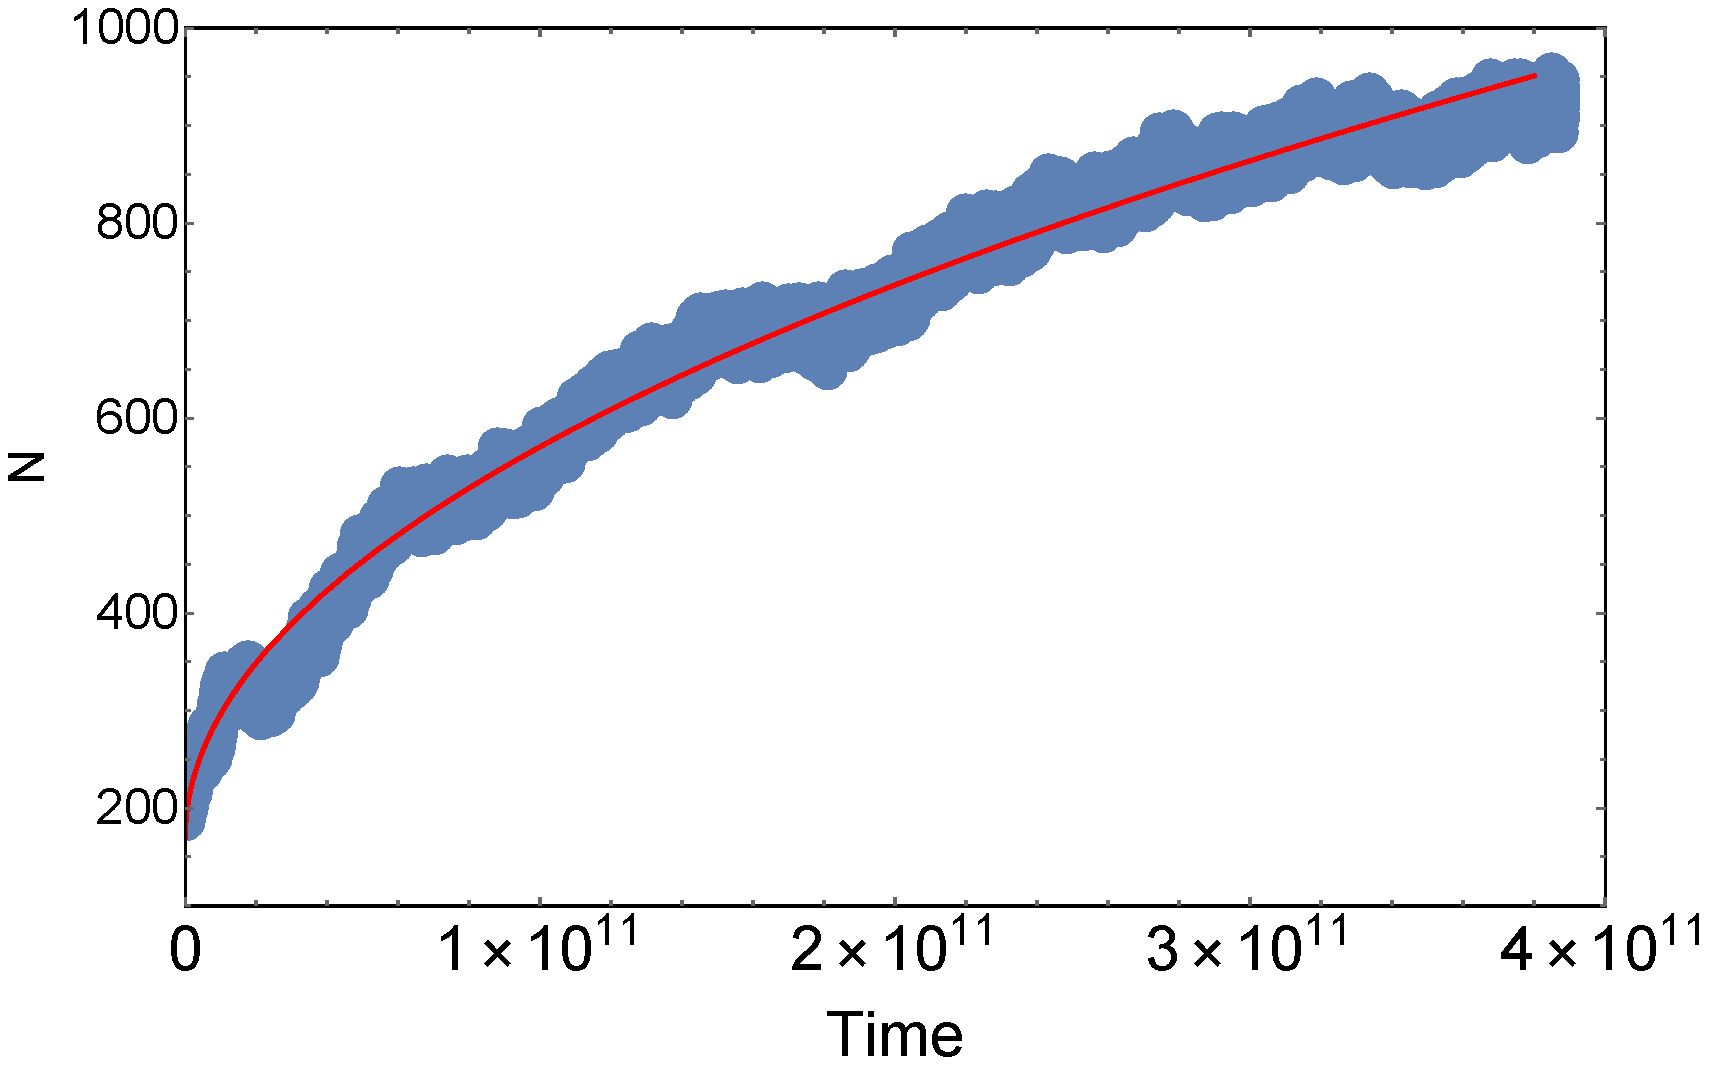
\includegraphics[scale=0.3]{Fig2.pdf}
\caption{$N$ vs. $t$. The growth rate here is for $\delta \mu = 0.17$ with $k_s=4$ and $k_\theta = 6$. The fit is $1.27*10^{-3}*\sqrt{t+2342}+170$}\label{fig:GrowthRate}
\end{figure}
\begin{figure}[tbp]
\centering
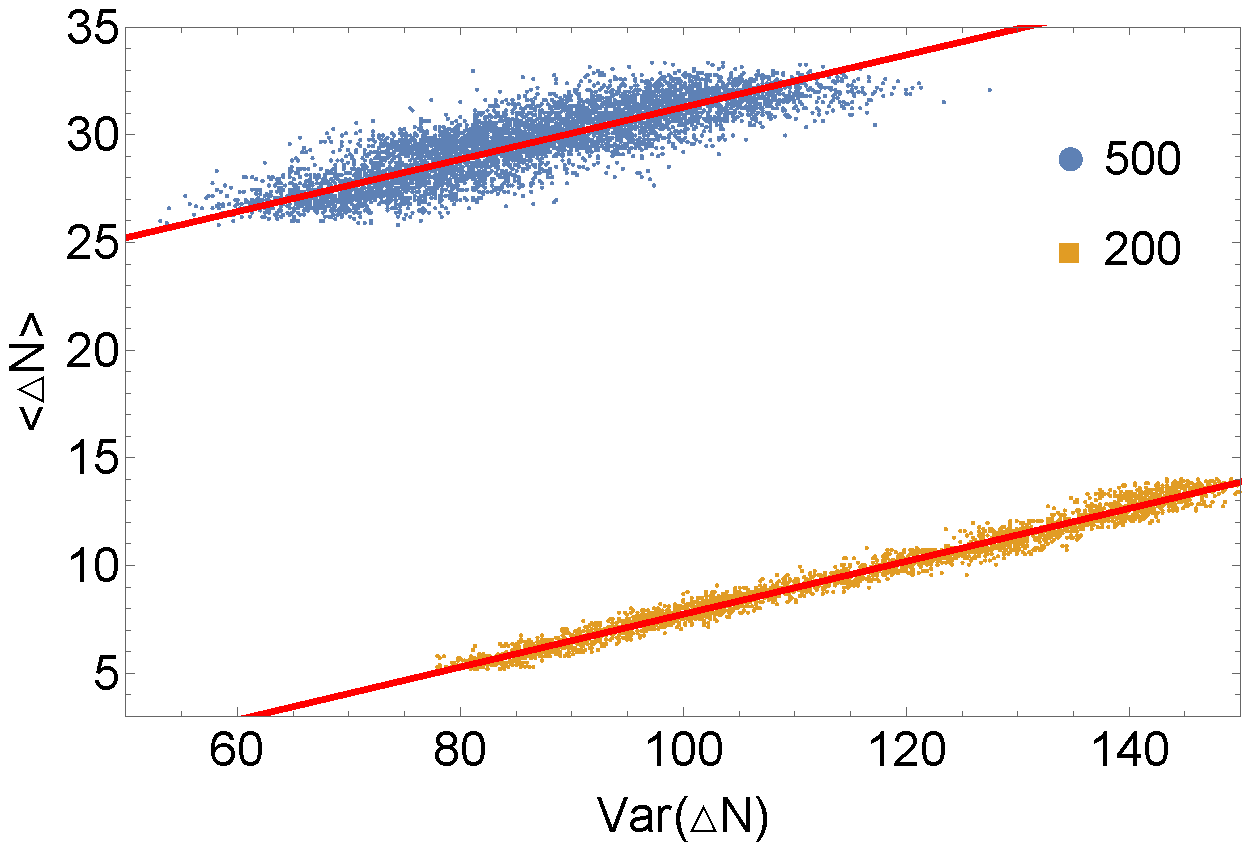
\includegraphics[scale=0.4]{Fig3.pdf}
\caption{$\Delta N$ vs. $Var(\Delta N)$ for different $N_0$. The blue dot is from measurements of 500s particle assemblies. The orange dot is from measurements of 200s particle assemblies. The slope extracted here is approximately 0.08 making $\frac{v}{D}=0.16$. The data here is for $\delta\mu=0.17$, $k_s=4$ and $k_\theta = 6$.} \label{fig:growthvsvariance}
\end{figure}


%\section{Small n modes deviation}
%The smallest n modes show some deviation from the Helfrich description as shown in the Fig.~\ref{fig:fit} . The deviation seems to be an apparent increase in the surface tension. This effect might be because the number of the particle $N$ in this simulations is always changing. Thus this might make difficult for the longest wavelength move to relax. In this paper, we have reported the $\gamma$ extracted from the bigger n modes. 
%\begin{figure}[tbb]
%\centering
%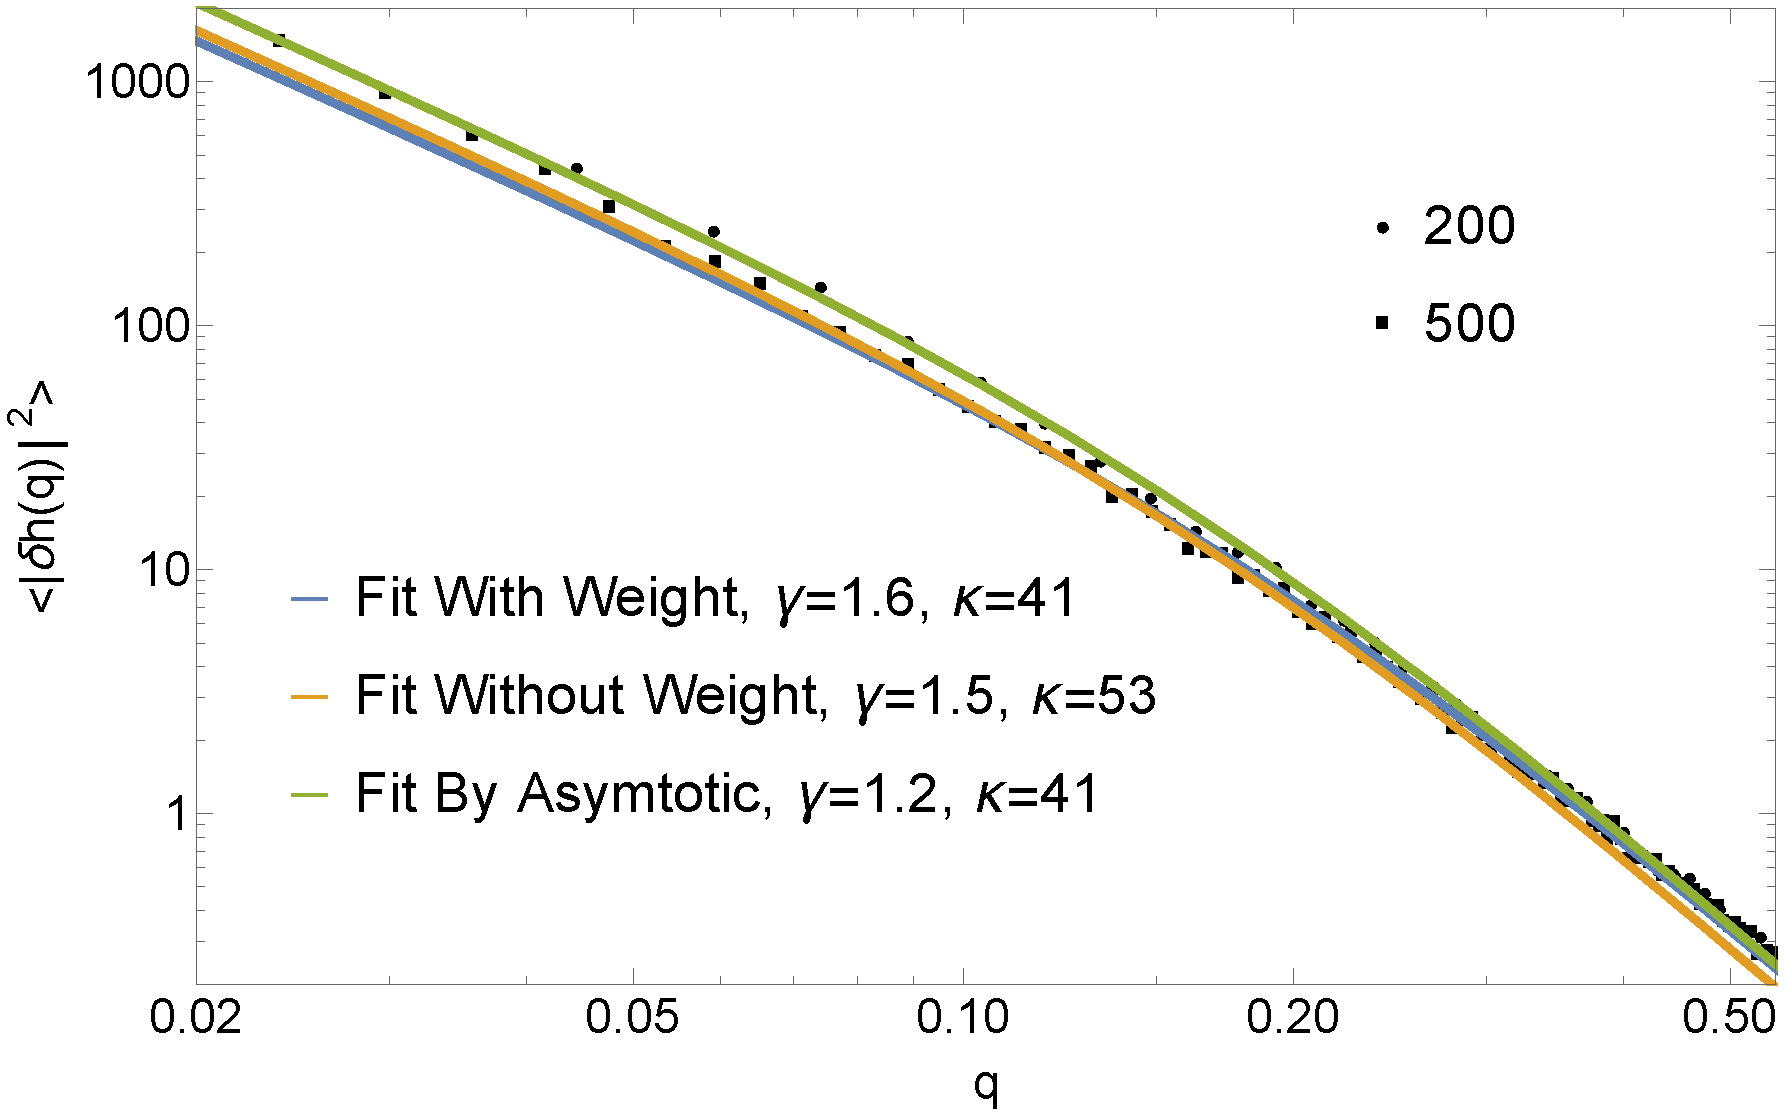
\includegraphics[scale=0.30]{fittingandsmallneffect.pdf}
%\caption{$\langle|\delta %h(q)|^2\rangle$ vs. $q$ for $\delta %\mu \approx 0$ with $k_s=4$ and %$k_\theta = 6$. For the smallest n %modes, both the 200 and 500 particles %spectrums converge to the $\gamma=1.2$ %while the rest of the n modes follow %$\gamma=1.6$ } \label{fig:fit}
%\end{figure}
%\section{Fitting Procedure}
%In order to extract $\gamma$ and $\kappa$ we need to fit $\langle|\delta h(q)|^2\rangle$ to $\frac{1}{\gamma q^2 +\kappa q^4}$. However, to fit the function correctly, we have to take into account that the variance of the spectrum is not constant. Specifically, the standard deviation of this spectrum is equal to its average. In order words, the errors in measuring in amplitude of the long wavelength modes will be significantly higher than the errors in measuring the amplitudes of the short wavelength ones. This is because each mode can be independently described with an exponential distribution. To fit the spectrum, we have to adjust the weight of the variances in the fitting procedure: $\rm{Weight(q)} = \frac{1}{\rm{Var(\langle|\delta h|\rangle ^2)}}$ so that we do not overfit the long wavelength region.

\section{4. Predicting effective elastic constants}

In the main text, we have used the bounds to answer the question: what is the required $\delta\mu$ to make the assembly acquire certain effective tension, $\gamma$. In a different way, we can use the bounds to address another question: given a $\delta\mu$, what is the least deviated from equilibrium, $\gamma$, the system will adopt. Fig~\ref{fig:epsilonpredict} shows how Eq. 7 and Eq. 8 in the main text answer this question.
\begin{figure}[tbb]
\centering
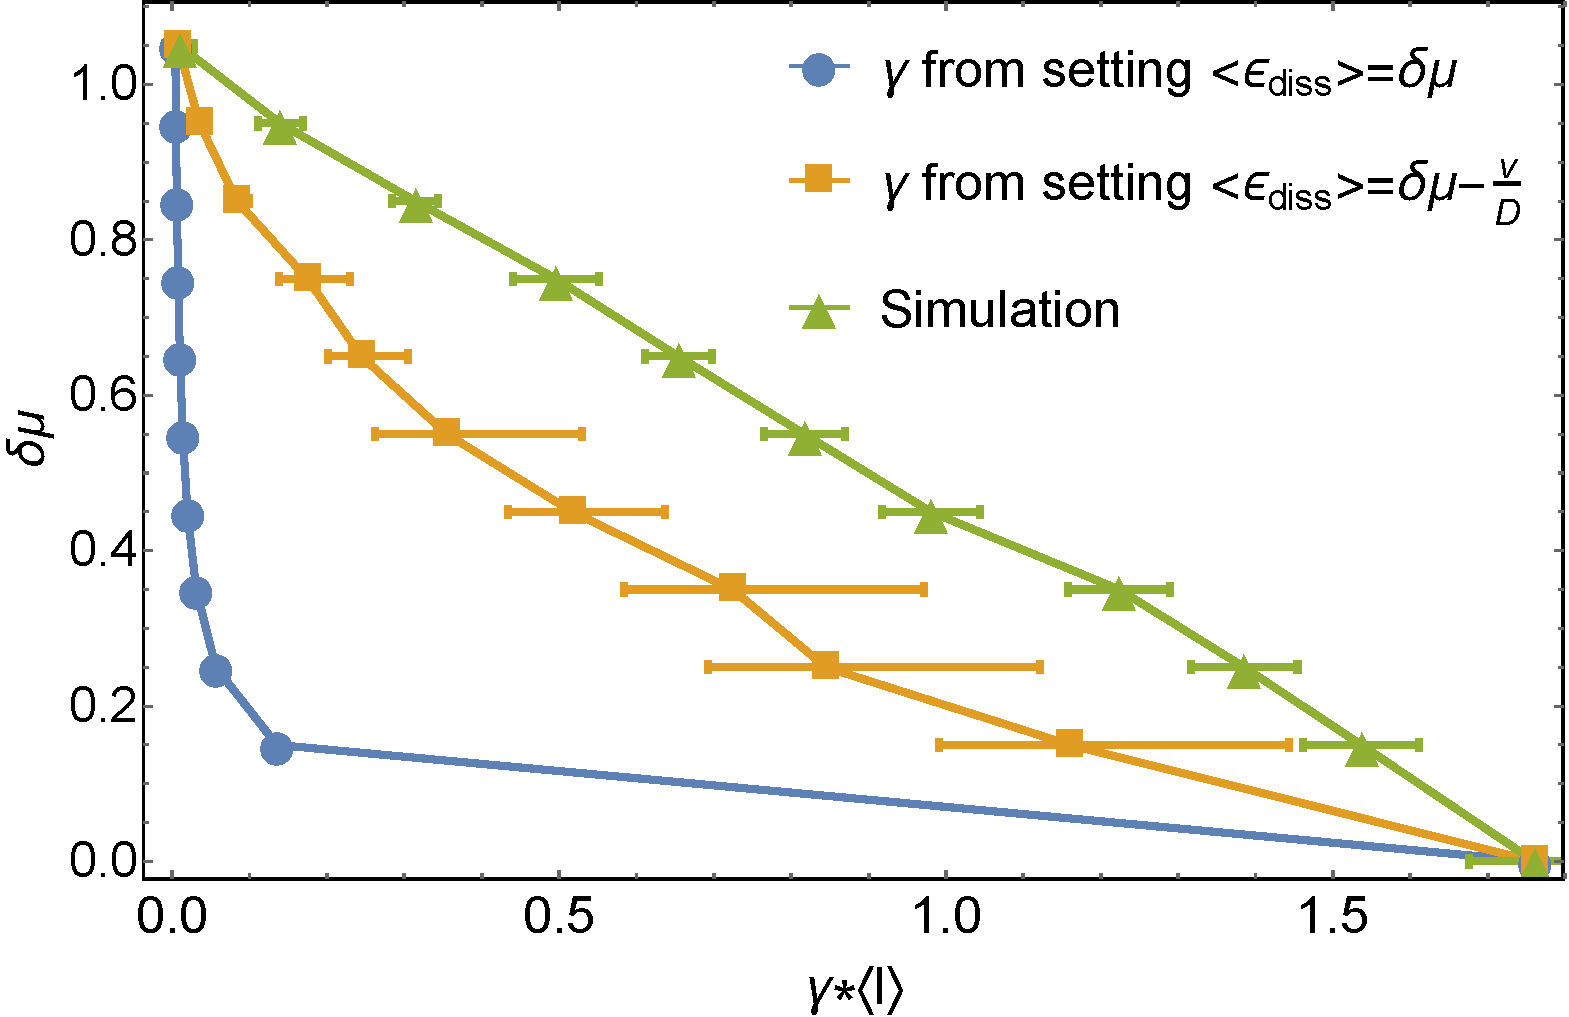
\includegraphics[scale=0.27]{Fig4.pdf}
\caption{$\delta\mu$ vs. $\gamma$. Instead of predicting the required $\delta\mu$, the blue curve (from Eq. 7) and the orange curve (from Eq. 8) can be used to predict the effective surface tension at certain $\delta \mu$. The data here is for $k_s=4$ and $k_\theta = 6$.} \label{fig:epsilonpredict}
\end{figure}


\section{5. Measurement of The Surface Tension and Bending Rigidity}

As stated in the main text, the fluctuation of $|\delta h(q)|^2$ follows  a Helfrich like Hamiltonian. This also means that the fluctuations of $|\delta h(q)|^2$ follow an exponential distribution as shown in Fig.~\ref{fig:expdistributionateq}. We find that this is also true even when the system is out of equilibrium (Fig.~\ref{fig:expdistributionaoutofeq}).

Since the distribution of $|\delta h(q)|^2$ is exponential, its standard deviation is the same as its average. This is a property of the exponential distribution. And since the average value of $|\delta h(q)|^2$ is proportional to $\frac{1}{(\gamma q^2+\kappa q^4)}$, the smaller q the bigger the average and its standard deviation will be. When fitting the power spectrum data to obtain estimates of $\gamma$ and $\kappa$, we accounted for the varying standard deviation by appropriately reweighting the errors in a q mode by its inverse magnitude. With this, the fit will not overvalue the contribution of the errors from the small q modes.
 
%Because of this, if one were to fit $\langle |\delta h(q)|^2\rangle$ to $q$ normally, they would get erroneous estimate for $\gamma$ and $\kappa$. This is because the lower $q$ modes have higher error naturally than the higher $q$ modes making normal fitting procedure overemphasizes on the lower $q$ modes to minimize the error.fol Fortunately, because we know each mode is exponential distributed , one simple way to correct this is by weighting the errors of the modes according to its inverse average magnitudes in the fit. We used the inverse average magnitudes because as stated above the standard deviations of the errors equal to the modes' average magnitudes. 
\begin{figure}
\centering
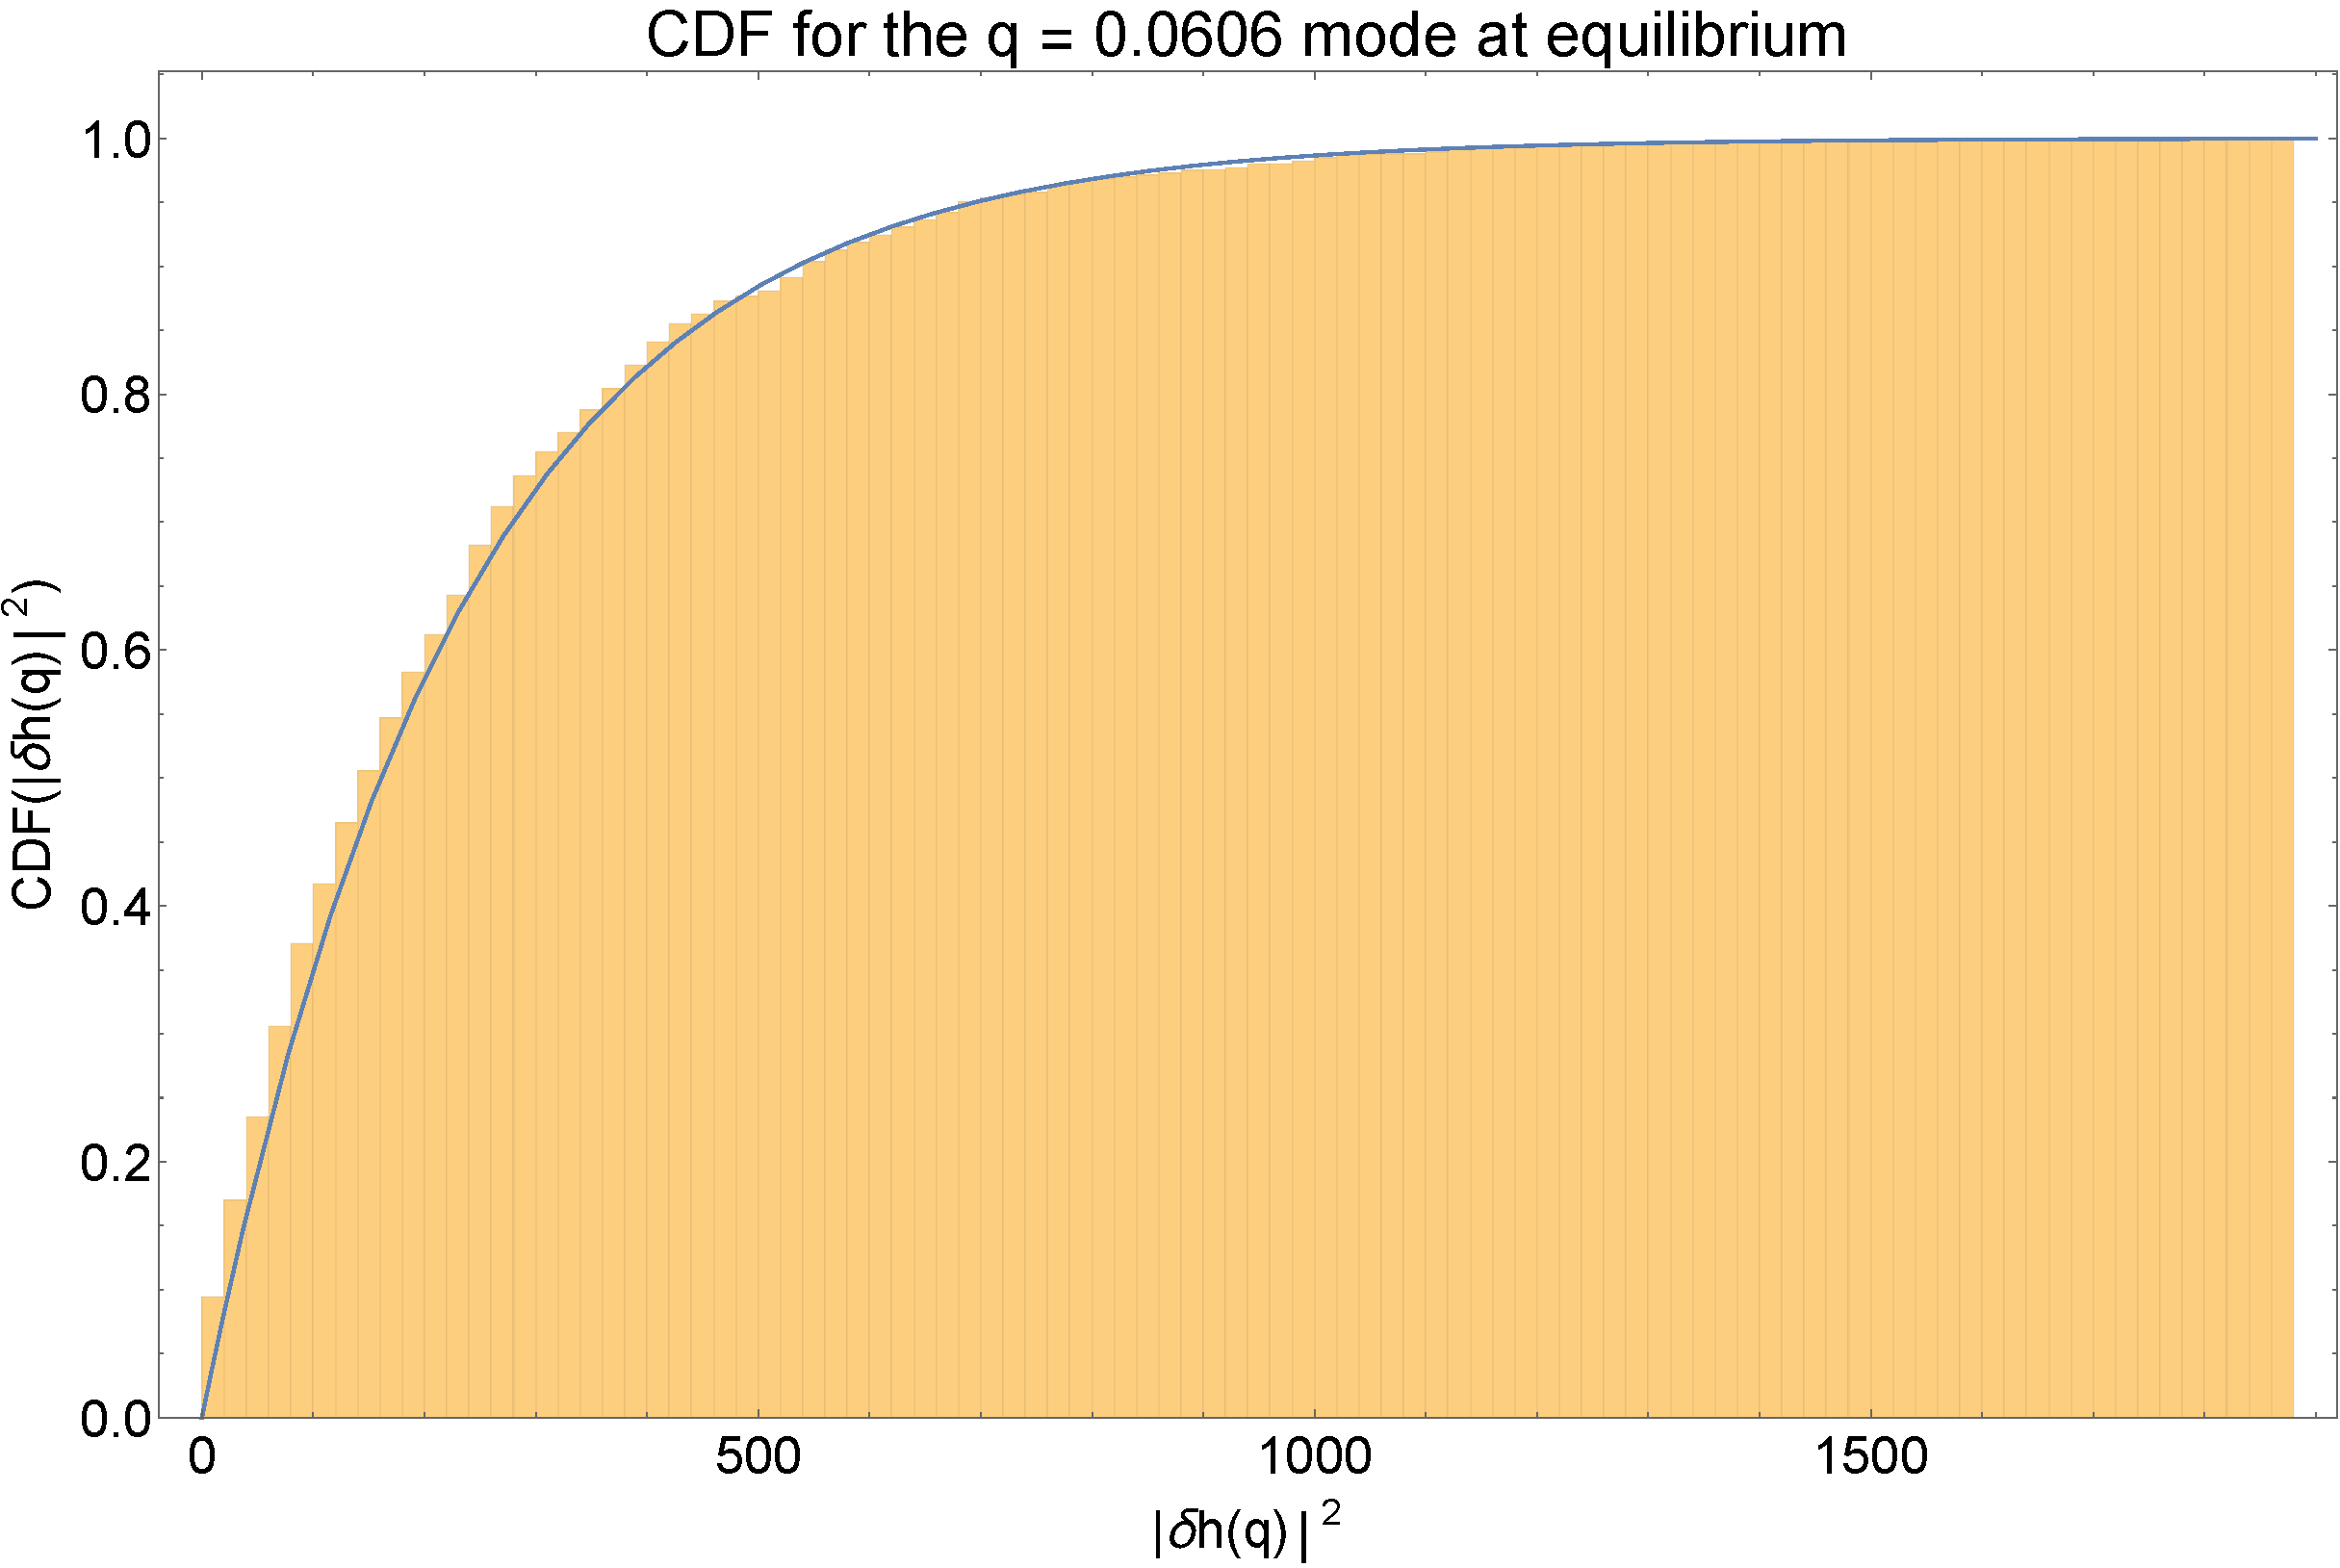
\includegraphics[scale=0.2]{Fig5.pdf}
\caption{The shaded region is the CDF of $|\delta h(q)|^2$ at q = 0.0606 obtained from simulations at equilibrium. The line is the CDF of the exponential distribution: $1-\exp{\frac{|\delta h(q)|^2}{\langle |\delta h(q)|^2\rangle_{\rm{sim}}}}$ here $\langle |\delta h(q)|^2\rangle_{\rm{sim}}$ is obtained from simulations. }  \label{fig:expdistributionateq}
\end{figure}
\begin{figure}
\centering
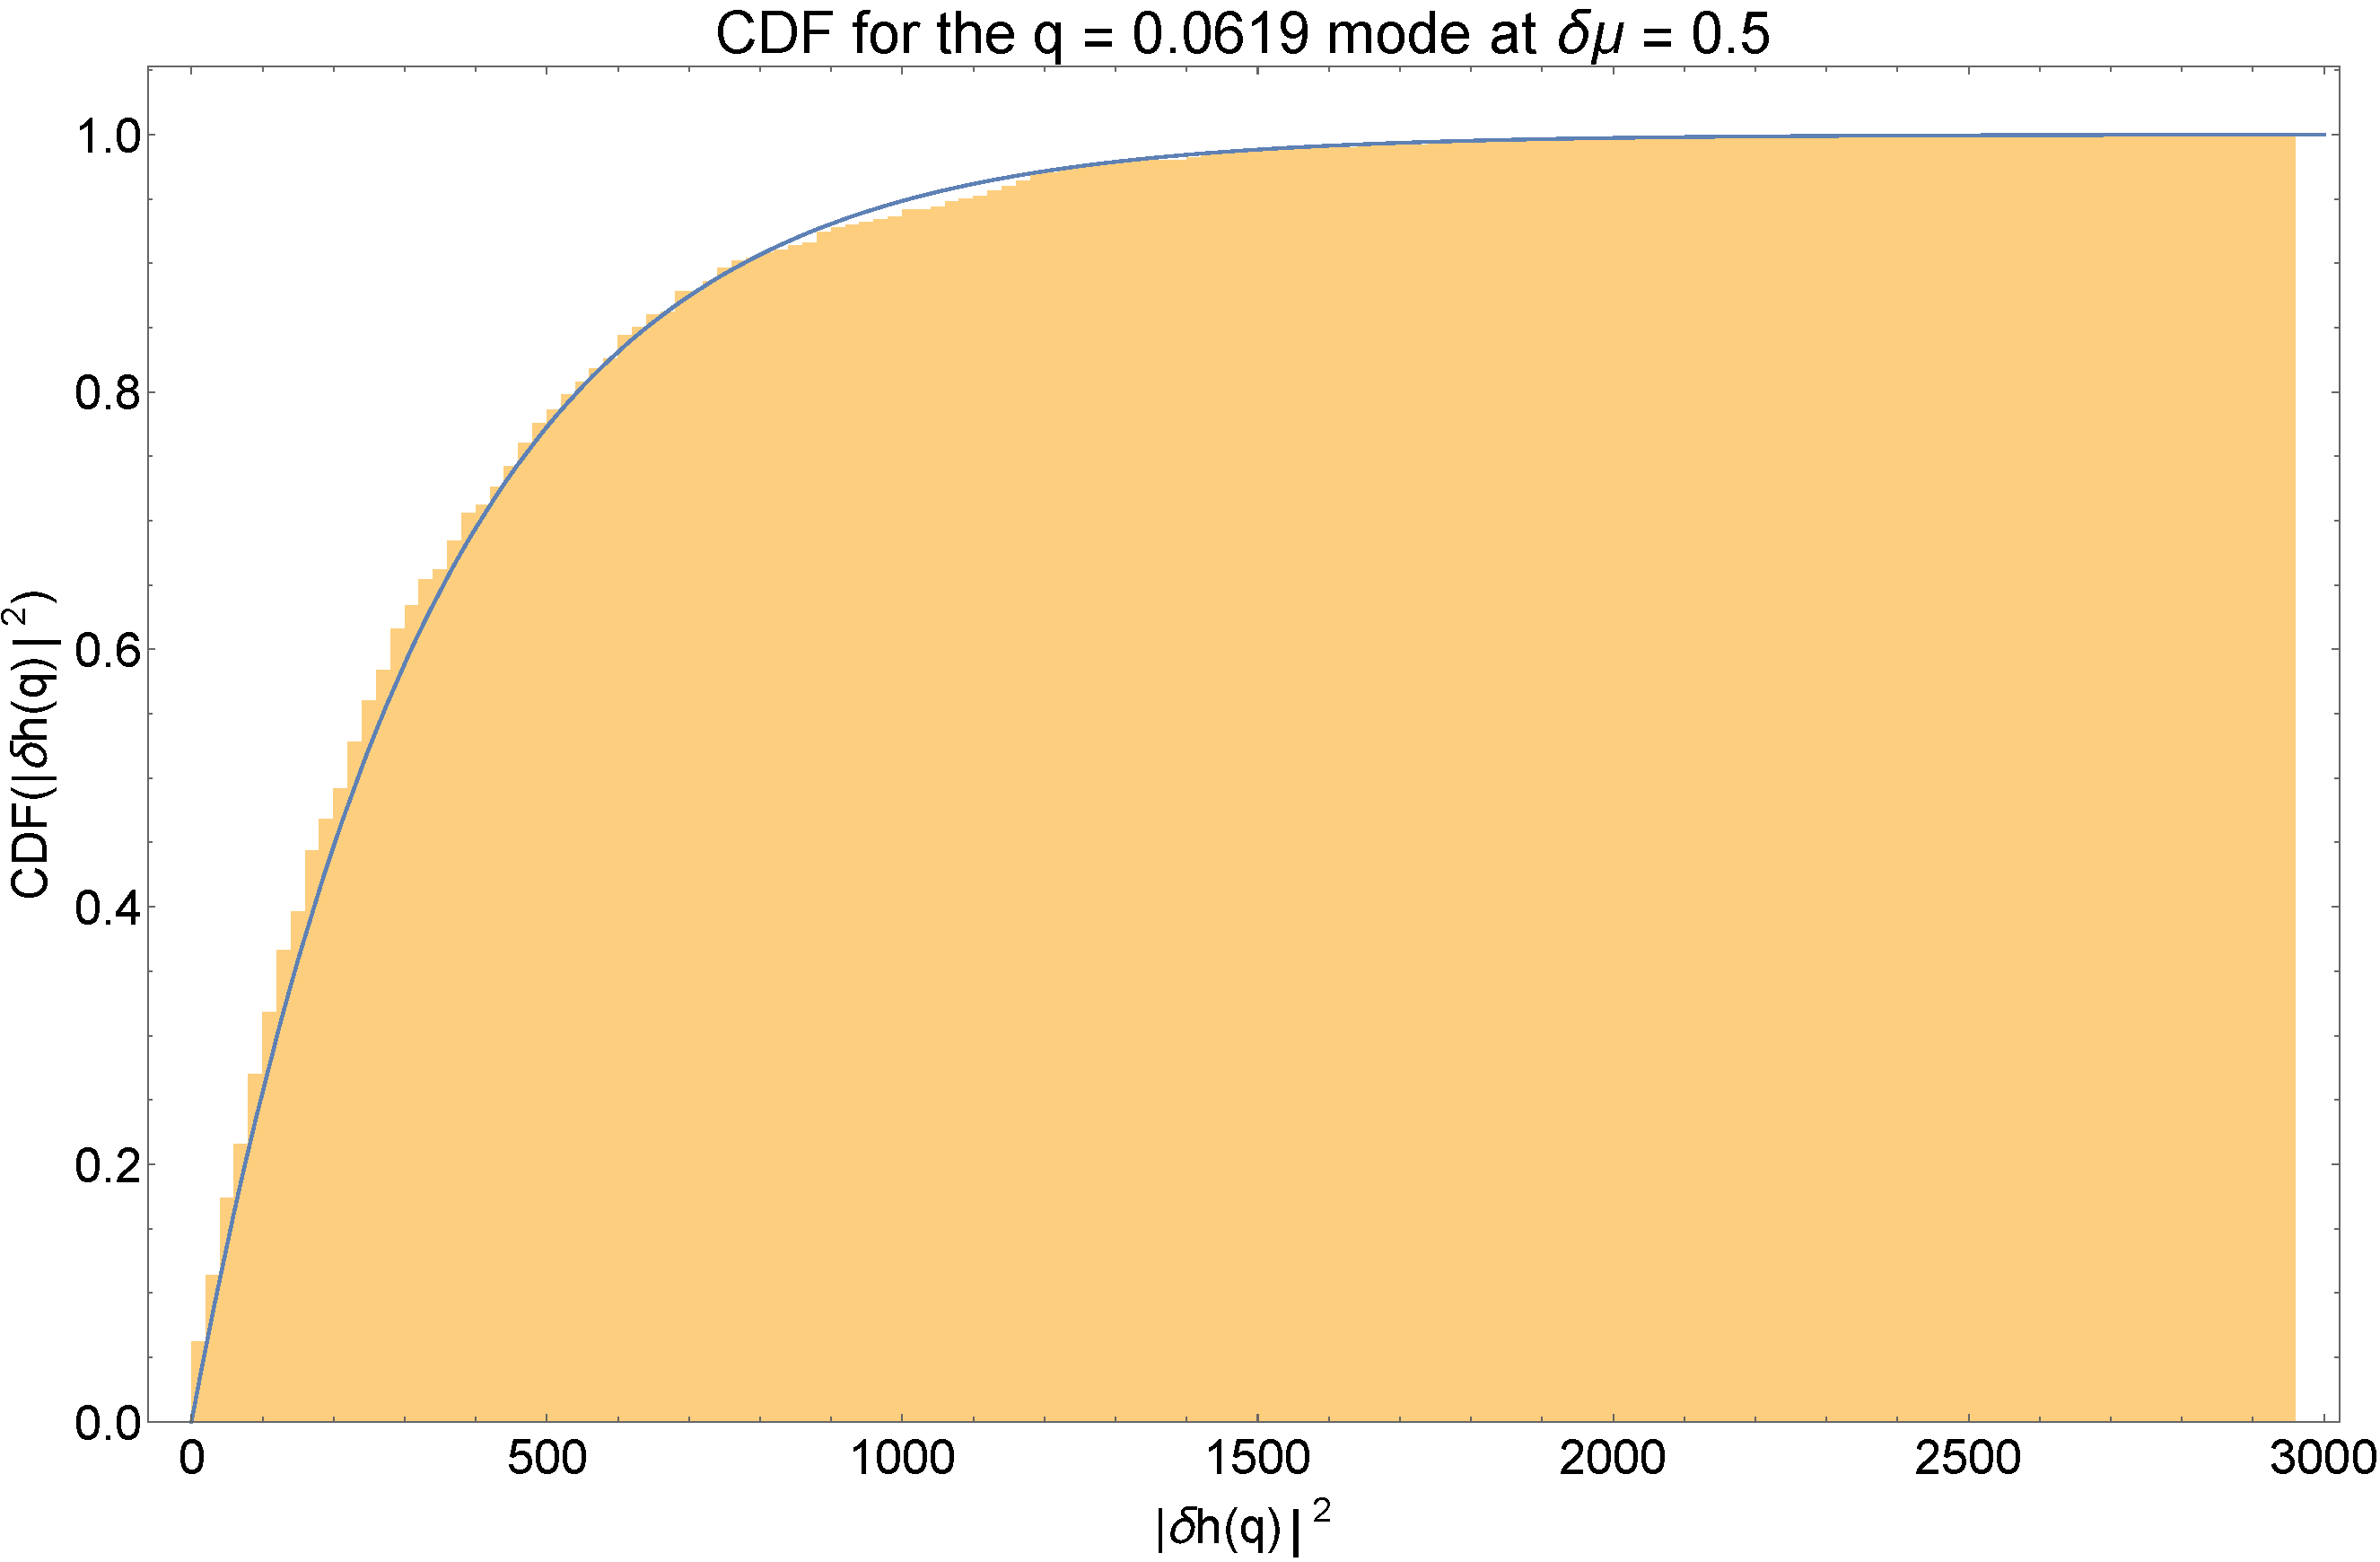
\includegraphics[scale=0.2]{Fig6.pdf}
\caption{The shaded region is the CDF of $|\delta h(q)|^2$ at q = 0.0619 obtained from simulations at $\delta\mu=0.5$ The line is the CDF of the exponential distribution: $1-\exp{\frac{|\delta h(q)|^2}{\langle |\delta h(q)|^2\rangle_{\rm{sim}}}}$ here $\langle |\delta h(q)|^2\rangle_{\rm{sim}}$ is obtained from simulations. }  \label{fig:expdistributionaoutofeq}
\end{figure}

\begin{figure}[tbb]
\centering
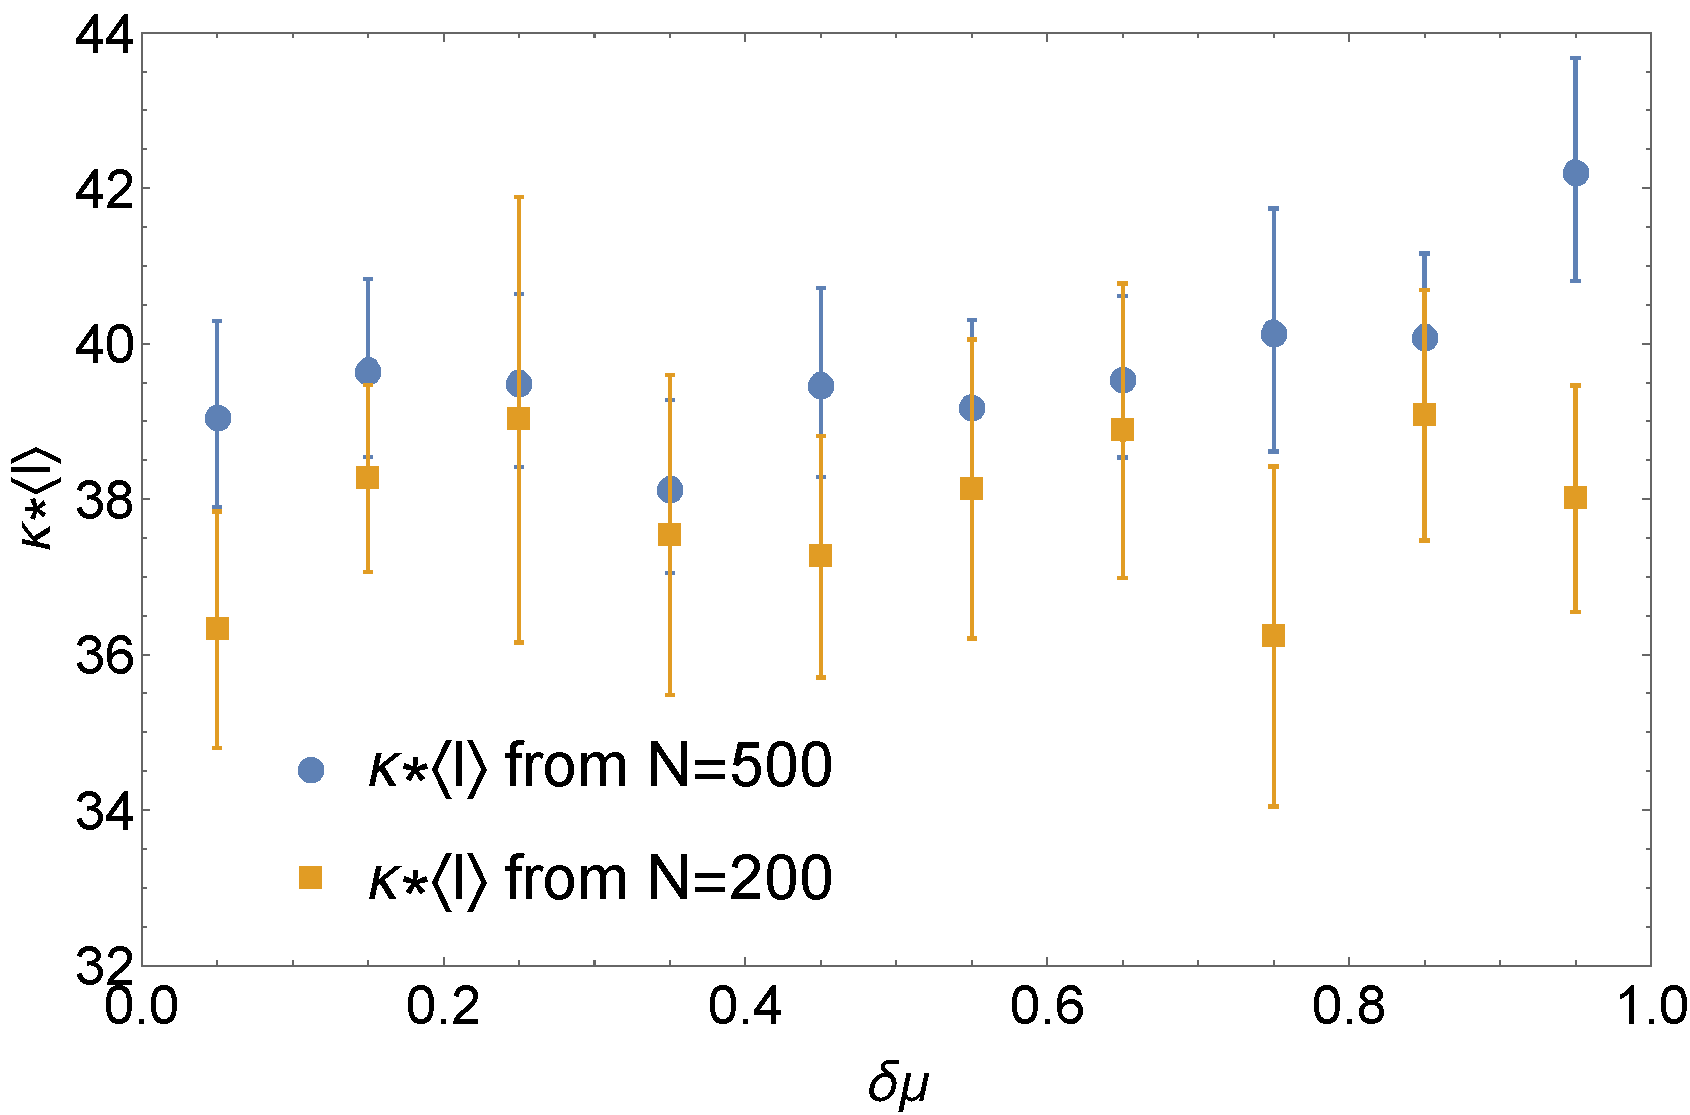
\includegraphics[scale=0.27]{Fig7.pdf}
\caption{$\kappa\langle l \rangle$ vs. $\delta\mu$. This graph shows how the bending rigidity , $\kappa$, changes with $\delta\mu$ from two different assembly's sizes. Unlike the surface tension which decreases with increasing $\delta\mu$, the bending rigidity does not change much from its equilibrium value. The data here is for $k_s=4$ and $k_\theta = 6$. The error bar represents the $95\%$ confidence interval from fitting.} \label{fig:bendingrigiditynormalization}
\end{figure}

\begin{figure}[tbb]
\centering
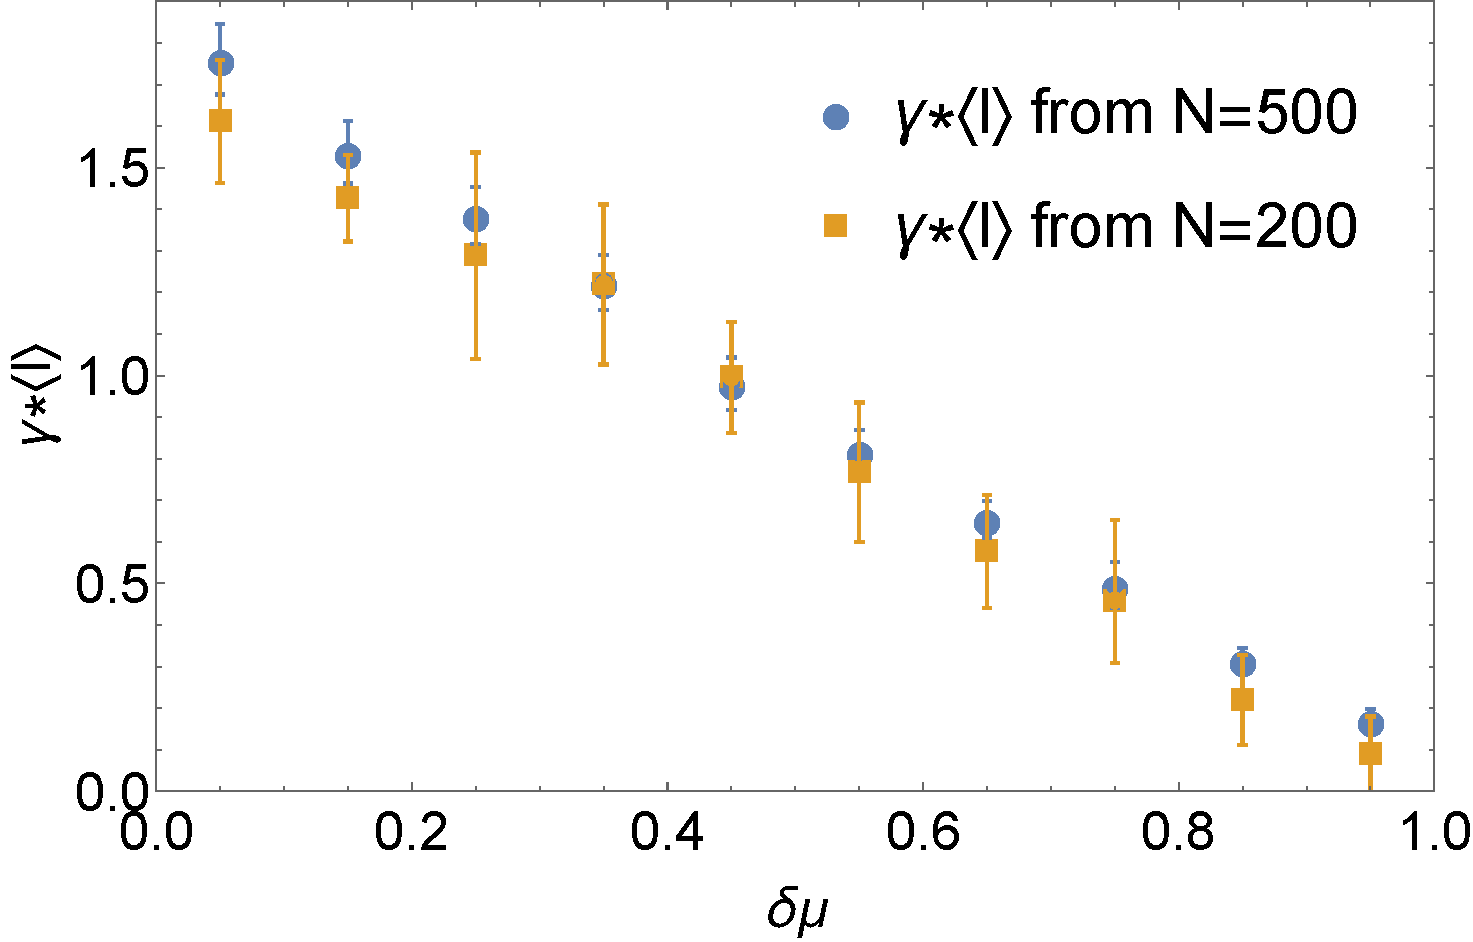
\includegraphics[scale=0.27]{Fig8.pdf}
\caption{$\gamma\langle l \rangle$ vs. $\delta\mu$. This graph shows how the surface tension , $\gamma$, changes with $\delta\mu$ from two different assembly's sizes. The data here is for $k_s=4$ and $k_\theta = 6$. The error bar represents the $95\%$ confidence interval from fitting.} \label{fig:surfacetensionynormalization}
\end{figure}

Fig.~\ref{fig:bendingrigiditynormalization} and \ref{fig:surfacetensionynormalization} show how the bending rigidity and the surface tension are normalized with increasing $\delta\mu$ respectively at two different system sizes. As stated in the main text, the surface tension decreases with increasing $\delta\mu$ and seems to be independent of size (Fig.~\ref{fig:surfacetensionynormalization}). Unlike the surface tension, the bending rigidity does not change much from its equilibrium value with increasing $\delta\mu$(Fig.~\ref{fig:bendingrigiditynormalization}). Within statistical error bars, the bending rigidity seems to independent of system size. Therefore, we have assume the bending rigidity a constant in our calculation of $\epsilon_{\rm{diss}}$


\section{6. A proof for the bounds in Eq.7 and Eq. 8 (Main Text) }
\begin{figure*}[tbp]
\includegraphics[width=1\linewidth,angle=0]{Fig9.pdf}
\caption{ Schematic of the addition/removal and rescaled moves of our Markov system. In our Markov network, to reach $\omega^\prime$ from $\omega$, the system has to go through an intermediate state $\tilde{\omega}$. From $\omega$ to $\tilde{\omega}$, a new particle is added to the assembly. From $\tilde{\omega}$ to $\omega^\prime$, a particle at the bottom is removed to preserve the same number of particles. We have colored the to be add or remove particle blue to distinguish it from the other particles in the assembly.}
\label{fig:MarkovSchematic}
\end{figure*}
Here we will detail the proof of Eq. 7 and Eq. 8 in the main text. In principle, we can start with a Markov state representation of the dynamics of the full ring and obtain expressions for the total entropy production in the non-equilibrium growth process. However, adapting or applying results such as the thermodynamic uncertainty relation to processes of this sort where the size of the system is not bounded and can increase, is potentially problematic due to the fact that time independent steady state properties are no longer guaranteed. Indeed, the thermodynamic uncertainty relations were derived for finite Markov state graphs, or for Markov state graphs with periodic boundary conditions~\cite{Barato2015,Gingrich2016}. 

We now show how these issues can be overcome in order to adapt thermodynamic uncertainty like relations to the membrane growth process considered in the main text. Towards this goal, we will focus on, and represent using a Markov process, the dynamics of a segment of the ring like assembly depicted in Fig.~\ref{fig:MarkovSchematic} as the membrane assimilates and gives up monomers. The ring like segment is assumed to be composed on $M$ beads with periodic conditions at the ends. A state $\omega$ of this segment can transition to a state $\omega^{\prime}$ after an addition event through a pathway of the sort depicted in Fig.~\ref{fig:MarkovSchematic}. Specifically, a particular monomer insertion event is allowed to take place with a rate $W_{\rm add}(\omega,\tilde{\omega})$ where $\tilde\omega$ denotes an intermediate state with $M+1$ beads. Since we are only interested in focusing on segments with $M$ beads, we then construct $\omega^\prime$ from $\tilde\omega$ by simply resolving the first $M$ beads in the clockwise direction without loss of generality. 

A transition from $\omega^\prime$ to $\omega$ due to a monomer reversal event proceeds according to the schematic in Fig~\ref{fig:MarkovSchematic}. Here, we first imagine extending the segment $\omega^\prime$ to construct a $M+1$ bead segment, $\tilde{\omega}$ by including the bead from the full membrane that is adjacent to the clockwise end of $\omega^\prime$. The probability associated with generating this intermediate configuration can be represented as $P(\tilde{\omega}|\omega^\prime)$ and depends on the correlations and steady state generated as the membrane is grown at a given value of $\delta \mu$. Next, a monomer removal event is allowed to take place with a rate $W_{\rm remove}(\tilde{\omega},\omega)$. 

As an aside, we note that this set of dynamics of the $M$ bead segment requires as an input the conditional probability $P(\tilde{\omega}|\omega^\prime)$. Alternately, one can imagine evolving the above described dynamics for a test conditional probability distribution $P_{\rm test}(\tilde{\omega}|\omega^\prime)$. For sufficiently large values of $M$, the steady state generated under the above described dynamics can be used to self consistently generate the conditional probability $P_{\rm ss}(\tilde{\omega}|\omega^\prime)$ where the subscript ${\rm ss}$ is meant to denote that the conditional probability has been generated by analyzing the steady state of the $M$ bead segment as follows. Imagine focusing on a subsection of the $M$ bead segment of size $L\gg 1$ and computing the probability of finding a bead adjacent to this subsection. For dynamics generated with the correct input conditional probability, $P(\tilde{\omega}|\omega^\prime)$, when $L,M\gg 1$ and the size of the $M$ bead segment is far greater than any correlation length in the system, the conditional probability computed from the $P$ bead subsection,$P_{\rm ss}(\tilde{\omega}|\omega^\prime)$, should closely resemble $P(\tilde{\omega}|\omega^\prime)$. For dynamics generated with a test conditional probability, $P_{\rm test}(\tilde{\omega}|\omega^\prime)$, the self consistency condition $P_{\rm test}(\tilde{\omega}|\omega^\prime)=P_{\rm ss}(\tilde{\omega}|\omega^\prime)$ can be used to progressively refine the input estimate. In this manner, the dynamics of the $M$ bead segment can potentially be used to obtain estimates of the correlations and steady states generated in the original non-equilibrium growth process. 


Given this description of dynamics, an expression for entropy production rate for a monomer absorption event resulting in a transition from a state $\omega$ to a state $\omega^\prime$ through an intermediate state $\tilde\omega$ is simply given by 

\begin{equation}
\label{eq:entprod}
\begin{split}
    &
    k_B^{-1}\dot{S}(\omega,\tilde\omega,\omega^\prime)=J_{\Delta N}(\omega,\tilde\omega,\omega^\prime)\ln\frac{P^M(\omega)W_{\rm add}(\omega,\tilde\omega)}{P^M(\omega^\prime)P(\tilde\omega|\omega^\prime)W_{\rm remove}(\tilde \omega,\omega)A}
\end{split}
\end{equation}
where
\begin{equation}
\begin{split}
    &J_{\Delta N}(\omega,\tilde\omega,\omega^\prime)\equiv\\& \frac{1}{M}\left[\frac{1}{A}P^M(\omega)W_{\rm add}(\omega,\tilde\omega)-P^M(\omega^\prime)P(\tilde\omega|\omega^\prime)W_{\rm remove}(\tilde \omega,\omega)\right]
\end{split}
\end{equation}
and we have used $P_M(\omega)$ to denote the steady state probability distribution associated with sampling the state $\omega$ in the $M$ bead segment. Note also that the conditional probability can be expressed as $P(\tilde \omega|\omega^\prime)=P(\tilde \omega,\omega^\prime)/P^M(\omega^\prime)$ where $P(\tilde \omega,\omega^\prime)$ is simply the joint probability associated with sampling $\tilde \omega$ and $\omega^\prime$. Since the $M$ bead segment $\omega^\prime$ is a subset of the $M+1$ bead segment $\tilde\omega$, the joint probability $P(\tilde \omega,\omega^\prime)$ can be compactly expressed using the symbol $P^{M+1}(\tilde \omega)$, the steady state probability distribution associated with sampling the $M+1$ length segment, $\tilde \omega$. 

To proceed, we note that the ratio of add and removal transition rates are informed by the microscopic dynamics and satisfy 
\begin{equation}
\label{eq:dB}
    \frac{W_{\rm add}(\omega,\tilde\omega)}{W_{\rm remove}(\tilde \omega,\omega)}=e^{\beta\left(\left[E^M_{\rm{eq}}(\omega)-E^{M+1}_{\rm{eq}}(\tilde\omega)\right]+\mu\right)}
\end{equation}
where $\beta^{-1}\equiv k_B T$ sets the thermal energy scale, $E^M_{\rm{eq}}(\omega)$ is the intrachain potential energy of the $M$ bead segment and $E^{M+1}_{\rm{eq}}(\tilde \omega)$ is the intrachain potential energy of the $M+1$ bead segment. The condition in Eq.~\ref{eq:dB} is consistent with the microscopic dynamics used in this paper. We also define $P_{\rm eq}^{M}(\omega)=\exp{-\beta E^M_{\rm{eq}}(\omega)}/Z^M_{\rm eq}$ where $Z^M_{\rm eq}=\sum_{\omega}\exp{-\beta E^M_{\rm{eq}}(\omega)}$ and $P_{\rm eq}^{M+1}(\tilde \omega)=\exp{-\beta E_{\rm eq}^{M+1}(\tilde\omega)}/Z^{M+1}_{\rm eq}$ where $Z^{M+1}_{\rm eq}=\sum_{\tilde\omega}\exp{-\beta E^{M+1}_{\rm eq}(\tilde \omega)}$. Formally, $P_{\rm eq}^M(\omega)$ and $P_{\rm eq}^{M+1}(\tilde \omega)$ denote the equilibrium Boltzmann probability distributions associated with the $M$ and $M+1$ segments, $\omega$ and $\tilde\omega$ respectively. 


Using these definitions and symbols, and using Eq.~\ref{eq:dB}, we can write Eq.~\ref{eq:entprod} as 
\begin{equation}
\label{eq:entprod2}
    \begin{split}
      k_B^{-1}\dot{S}(\omega,\tilde\omega,\omega^\prime)&=J_{\Delta N}(\omega,\tilde\omega,\omega^\prime)\left[\ln\frac{P^M(\omega)}{P_{\rm eq}^M(\omega)}-\ln\frac{P^{M+1}(\tilde\omega)}{P_{\rm eq}^{M+1}(\tilde\omega)}\right]\\&+J_{\Delta N}(\omega,\tilde\omega,\omega^\prime)\beta\delta \mu
    \end{split}
\end{equation}
where $\delta \mu\equiv \mu- (F^{M+1}_{\rm eq}-F^M_{\rm eq})-\beta^{-1}\rm{ln}A$ where $F^{M+1}_{\rm eq}=-\beta^{-1}\ln Z^{M+1}_{\rm eq}$ and $F^{M}_{\rm eq}=-\beta^{-1}\ln Z^{M}_{\rm eq}$, is the excess chemical potential driving the non-equilibrium growth process. 
To get an expression for the overall entropy production rate, we now sum over all possible transitions. Since every allowed transition between a pair of states $\omega$ and $\omega^\prime$ has an unique $M+1$ bead intermediate state, $\tilde \omega$, the sum over allowed transitions is formally equivalent to summing over all possible pairs of $M$ and $M+1$ bead states, $\omega$ and $\tilde\omega$. 

Performing this summation, an expression for the total entropy production can be written as 
\begin{equation}
\begin{split}
    k_B^{-1}\dot{S}&=\beta\langle \dot{N} \rangle \delta \mu+\sum_{\omega} \ln\frac{P^M(\omega)}{P_{\rm eq}^M(\omega)}\sum_{\tilde\omega} J_{\Delta N}(\omega,\tilde\omega)\\&-\sum_{\tilde\omega} \ln\frac{P^{M+1}(\tilde\omega)}{P_{\rm eq}^{M+1}(\tilde \omega)}\sum_{\omega} J_{\Delta N}(\omega,\tilde\omega)
\end{split}
\end{equation}
where we have dropped the dependence of $J$ on $\omega^\prime$ for ease of notation and we have used the fact that the sum of all currents $J$ is simply the net average rate of growth, $\langle \dot{N}\rangle$.  
To proceed further, we note that $\sum_{\omega} J_{\Delta N}(\omega,\tilde\omega)$ is equal to the net rate at which the $M+1$ bead configuration $\tilde\omega$ is generated from a monomer insertion event. We make the mean field assumption that this net rate of generation is in fact proportional to the steady state probability $P^{M+1}(\tilde \omega)$, $\sum_{\omega} J_{\Delta N}(\omega,\tilde\omega)\approx \langle \dot{N}\rangle P^{M+1}(\tilde \omega)$. Similarly, using this mean field assumption and the condition of probability flux conservation, we can write $\sum_{\tilde\omega} J_{\Delta N}(\omega,\tilde\omega)\approx \langle \dot{N}\rangle P^M(\omega)$. With these mean field assumptions, the expression for entropy production reads 
\begin{equation}
\label{eq:entprod3}
\begin{split}
    &k_B^{-1}\dot{S}=\dot{\langle N\rangle}\lbrack\beta\delta\mu -(D[P^{M+1}(\tilde \omega)|| P_{\rm eq}^{M+1}(\tilde \omega)]\\
    &-D[P^{M}(\omega)|| P_{\rm eq}^{M}(\omega)])\rbrack
\end{split}
\end{equation}
where $D[p||q]$ denotes the relative entropy between distributions $p$ and $q$. Finally, noting the fact that $D[P^{M+1}(\tilde \omega)|| P_{\rm eq}^{M+1}(\tilde \omega)]$ and $D[P^{M}(\omega)|| P_{\rm eq}^{M}(\omega)]$ are relative entropies between non-equilibrium and equilibrium distributions of segements of lenght $M+1$ and $M$ respectively, and using 
\begin{equation}
\begin{split}
    &D[P^{M+1}(\tilde \omega)|| P_{\rm eq}^{M+1}(\tilde \omega)]-D[P^{M}(\omega)|| P_{\rm eq}^{M}(\omega)]\\&\approx \frac{D[P^{M}(\omega)|| P_{\rm eq}^{M}(\omega)]}{M}
\end{split}
\end{equation}
in the limit $M\gg 1$
we can write Eq.~\ref{eq:entprod3} as 
\begin{equation}
\label{eq:entprod4}
    k_B^{-1}\dot{S}=\dot{\langle N\rangle}\left[\beta\delta \mu -\frac{D[P^{M}(\omega)|| P_{\rm eq}^{M}(\omega)]}{M}\right]
\end{equation}
and since $\dot{\langle N\rangle}\geq 0$ for all our cases, the second law of thermodynamics requires that:
\begin{equation}
\label{eq:equation7maintex}
    \delta \mu -\frac{D[P^{M}(\omega)|| P_{\rm eq}^{M}(\omega)]}{\beta M}\geq 0
\end{equation}
Finally, by define a new energy $E_{\rm{eff}}^M(\omega)$ with: $P^M(\omega)\equiv\exp{-\beta E_{\rm{eff}}^M(\omega)}/Z^M_{\rm{eff}}$ and $F^M_{\rm{eff}}=-\beta^{-1} \ln Z^M_{\rm{eff}} = -\beta^{-1}\ln \sum_\omega \exp{-\beta E_{\rm{eff}}^M(\omega)}$ we can rewrite the Eq.~\ref{eq:equation7maintex} as:
\begin{equation}
\label{eq:equation7maintex2}
    \delta \mu -\frac{\langle E^M_{\rm{eq}}-E^M_{\rm{eff}}\rangle_N+F^M_{\rm{eff}}-F^M_{\rm{eq}}}{M}\geq 0
\end{equation}
which is precisely the Eq. 7 in the main text derived from phenomenological considerations. Here $\langle... \rangle_N$ is averaging over the new energy $E_{\rm{eff}}^M$ landscape.

Even in regimes where the mean field assumption above is not applicable, similar expressions for the dissipation rate can be obtained. In these regimes, we write $P^{M+1}(\tilde \omega)$, $\sum_{\omega} J_{\Delta N}(\omega,\tilde\omega)\equiv \langle \dot{N}(\tilde \omega)\rangle P^{M+1}(\tilde \omega)$ and $\sum_{\tilde\omega} J_{\Delta N}(\omega,\tilde\omega)\equiv \langle \dot{N} (\omega)\rangle P^M(\omega)$ where we have defined $\langle \dot{N}(\omega) \rangle$ and  $\langle \dot{N} ({\tilde \omega}) \rangle$ as the average rate at which configurations $\omega$ and $\tilde \omega$ are generated. With these definitions, and assuming that $\langle\dot{N}(\omega)\rangle\geq 0$ for all configurations, Eq.~\ref{eq:entprod3} becomes 
\begin{equation}
\label{eq:entprod33}
\begin{split}
    &k_B^{-1}\dot{S}=\dot{\langle N\rangle}\lbrack\beta\delta\mu -(D[g(\tilde\omega)
    P^{M+1}(\tilde \omega)|| P_{\rm eq}^{M+1}(\tilde \omega)]\\
    &-D[g(\omega)P^{M}(\omega)|| P_{\rm eq}^{M}(\omega)]+g(\tilde\omega)
    P^{M+1}(\tilde \omega)\ln(g(\tilde\omega))\\
    &-g(\omega)P^{M}(\omega)\ln(g(\omega)))\rbrack
\end{split}
\end{equation}
where $g(\omega)\equiv \langle \dot{N}(\omega) \rangle/\langle\dot{N}\rangle$ and $\langle\dot{N}\rangle=\sum_\omega P^M(\omega) \langle\dot{N}(\omega)\rangle$. With these definitions and with the assumption that $\langle\dot{N}(\omega)\rangle\geq 0$ for all configurations, the combination $g(\omega)P^{M}(\omega)$ can be treated as a normalized probability distribution. The expression for entropy production in Eq.~\ref{eq:entprod33} explicitly accounts for correlations in the growth rate and configuration fluctuations. In the limit that $\langle \dot{N} (\omega)\rangle \approx \langle \dot{N}\rangle$, we recover the mean field expression in Eq.~\ref{eq:entprod4}. 

As mentioned earlier, by focusing on a ring segment with a finite $M$ beads instead of the whole assembly, we can write down a finite periodic Markov network for the segment. This then allows us to import the proof of the thermodynamics uncertainty relations which has been previously proven for arbitrary periodic Markov network~\cite{Barato2015,Gingrich2016}. The thermodynamics uncertainty relation states that:
\begin{equation}
\label{eq:thermodynamicsuncertaintyrelation}
    k_B^{-1}\dot{S}\geq\frac{J_\alpha^2}{ D_\alpha}
\end{equation}
Here $J_\alpha$ is any current of the Markov network and $D_\alpha$ is its diffusion constant. If we use the particle current $J_\alpha=\dot{\langle N \rangle}$ and plug in Eq.~\ref{eq:entprod4} then we have:
\begin{equation}
\label{eq:equation8maintext}
    \delta \mu -\frac{\langle E^M_{\rm{eq}}-E^M_{\rm{eff}}\rangle_N+F^M_{\rm{eff}}-F^M_{\rm{eq}}}{M}\geq \frac{\dot{\langle N \rangle}}{\beta D_N}
\end{equation}
which is Eq. 8 in the main text.
%P(l_{BE},l_{EC},l_{BC},\widehat{BEC},\widehat{ABE},\widehat{ECD},\widehat{ABC},\widehat{BCD})
% P(l_{BC},\widehat{ABC},\widehat{BCD})
%
%\begin{figure*}
%\centering
%  \subfloat[]{%
%   \includegraphics[scale=0.35]{estimationfordeltamu0d1ver2.pdf}}\hfill
% \subfloat[]{%
%    \includegraphics[scale=0.35]{estimationfordeltamu0d4ver2.pdf}}\\
%  \subfloat[]{
%   \includegraphics[scale=0.35]{estimationfordeltamu0d7ver2.pdf}}\hfill
%  \subfloat[]{%
%    \includegraphics[scale=0.35]{estimationfordeltamu1d0ver2.pdf}}\hfill
%\caption{Comparison of the Fourier Spectrums of the interface's fluctuation at different $\delta\mu$ from simulations and predicted by Eq. 8 in the main text. The data here is for $k_s=4$ and $k_\theta = 6$.} \label{fig:predictandsimulation}
%\end{figure*}
\section{7. Derivation of Eq. 9 in the main text}
Here we will detail how we write down Eq. 9 in the main text. As mentioned in the main text, we have approximated that the fluctuations of the system follow the Helfrich Hamiltonian with a normalized surface tension, $\gamma$. From simulations (see Fig.~\ref{fig:bendingrigiditynormalization}), the normalization of the bending rigidity, $\kappa$, is minimal. Thus, we will further assume that $\kappa= \kappa_{\rm eq}$ to make the calculation simpler. With this approximation, we have $\langle E_{\rm eq}\rangle _N=\langle l \rangle\sum_q\left(\frac{1}{2}\gamma_{\rm eq} q^2+\frac{1}{2}\kappa_{\rm eq} q^4\right)|\delta h(q)|^2$, $\langle E_{\rm eff}\rangle_N=\langle l \rangle\sum_q\left(\frac{1}{2}\gamma q^2+\frac{1}{2}\kappa_{\rm eq} q^4\right)|\delta h(q)|^2$ and $|\delta h(q)|^2=\frac{k_B T}{\langle l \rangle  \left(\gamma q^2+\kappa_{\rm eq}q^3\right)}$ . If we convert the sum here to integral using $dq=\frac{2\pi}{L}$:
\begin{equation}
    \langle E_{\rm eq}\rangle_N=\frac{L k_BT}{4\pi}\int_0^{2\pi/\lambda}\frac{\gamma_{\rm eq}q^2+\kappa_{\rm eq}q^4}{\gamma q^2+\kappa_{\rm eq}q^4}dq
\end{equation}

Here $\lambda$ is the smallest wavelength allowed by the assembly which we will take to be $\langle l \rangle \approx l_0$. With some algebra we will have:
\begin{equation}
    \langle E_{\rm eq}\rangle_N=\frac{N k_BT}{2}\left(1 - \frac{\lambda(\gamma-\gamma_{\rm eq})\rm{arctan}\left[\frac{2\pi\sqrt{\kappa_{\rm eq}}}{\sqrt{\gamma}\lambda}\right]}{2\pi\sqrt{\gamma\kappa_{\rm eq}}}\right)
\end{equation}
We have used: $N=\frac{L}{\langle l \rangle}=\frac{L}{ \lambda }$.The same procedure with $E_{\rm eff}$ yields:
\begin{equation}
    \langle E_{\rm eff}\rangle_N=\frac{N k_BT}{2}
\end{equation}
The free energy is $F_{\rm eff} = -k_BT\rm{ln}\left(\int \exp\left[-E_{\rm{eff}}(\delta h)\right]\delta h\right)$. Here if we plug in $E_{\rm eff}$ and realize that the integral of $\delta h$ is a Gaussian integral, we can simplify the free energy to:
\begin{equation}
\begin{split}
    F_{\rm eff}&= -k_BT\rm{ln}\left(\prod_q\frac{2\pi}{\gamma q^2+\kappa_{\rm eq} q^4}\right)^{(1/2)}\\
&=\frac{ -k_BT}{2}\sum_q\rm{ln}\left(\frac{2\pi}{\gamma q^2+\kappa_{\rm eq} q^4}\right)
\end{split}
\end{equation}
We then use similar procedure as in the case of $E_{\rm eq}$ to turn the sum into an integral. With a few line of algebras, we will obtain:
\begin{equation}
\begin{split}
     &F_{\rm eff}=\frac{N k_BT\lambda}{2\pi} \biggl(\sqrt{\frac{\gamma}{\kappa_{\rm eq}}}\rm{arctan}\left[\frac{2\pi}{\lambda}\sqrt{\frac{\kappa_{\rm eq}}{\gamma}}\right]\\
     &-\frac{\pi}{\lambda}\left(2+\rm{ln}\left[\frac{2\pi\lambda^2}{4\pi^2\kappa_{\rm eq}+\gamma\lambda^2}\right]\right)\biggr)
\end{split}
\end{equation}
Similarly, the expression for the $F_{\rm eq}$ is:
\begin{equation}
\begin{split}
     &F_{\rm eq}=\frac{N k_BT\lambda}{2\pi}\biggl(\sqrt{\frac{\gamma_{\rm eq}}{\kappa_{\rm eq}}}\rm{arctan}\left[\frac{2\pi}{\lambda}\sqrt{\frac{\kappa_{\rm eq}}{\gamma_{\rm eq}}}\right]\\
     &-\frac{\pi}{\lambda}\left(2+\rm{ln}\left[\frac{2\pi\lambda^2}{4\pi^2\kappa_{\rm eq}+\gamma_{\rm eq}\lambda^2}\right]\right)\biggr)
\end{split}
\end{equation}
If we plug in the definition of $\langle\epsilon_{\rm diss}\rangle:$
\begin{equation}
    \begin{split}
        \langle\epsilon_{\rm diss}\rangle&=\frac{\langle E_{\rm{eq}}-E_{\rm{eff}}\rangle_N+F_{\rm{eff}}-F_{\rm{eq}}}{N}\\
        &=\frac{k_BT\lambda}{4\pi}\biggl( \frac{(\gamma+\gamma_{\rm eq})\rm{arctan}[\frac{2\pi\sqrt{\kappa_{\rm eq}}}{\lambda\sqrt{\gamma}}]}{\sqrt{\gamma\kappa_{\rm eq}}}\\
        &- \frac{(2\sqrt{\gamma_{\rm eq}\gamma})\rm{arctan}[\frac{2\pi\sqrt{\kappa_{\rm eq}}}{\lambda\sqrt{\gamma_{\rm eq}}}]}{\sqrt{\gamma\kappa_{\rm eq}}} \\
        & -\frac{2\pi\left(\rm{ln}\left[\frac{4\pi^2\kappa_{\rm eq}+\gamma_{\rm eq}\lambda^2}{4\pi^2\kappa_{\rm eq}+\gamma\lambda^2}\right]\right)}{\lambda}\biggr)
    \end{split}
\end{equation}
which is Eq. 10 in our main text.
\section{8. 3D Model Membrane Simulation}

In this section, we detail calculations that qualitatively suggest that the results obtained with the 2D model in the main text can be extended to non-equilibrium growth problems with three dimensional vesicles/membranes. Following Ref.~\cite{Mahadevan2019}, we model a three dimensional fluid vesicle using a triangulated mesh. The nodes of the mesh are meant to represent membrane particles in a coarse-grained fashion. The energy associated with a specific configuration of the vesicle is given by  $H=\sum_{\rm faces}\left[ (k_A(A-A_0)^2 +\sum_{i=1}^3 k_\theta (\theta_i-\pi/3)^2 + \sum^\prime k_\phi (\phi-\pi)^2)\right]$, where $\sum_{\rm faces}$ is a sum over the triangulated faces, $A$ is the area of a triangulated face, $\theta_i$ are the angles inside a triangulated face,  $\sum^\prime$ denotes a sum over different adjacent phases and $\phi$ denotes the angle between two adjacent faces. 

In our model, the number of bonds or connections a particular particle can make is limited from $5$ to $7$.  Similar to the 2D model, we attempt to add and remove particle in our Monte Carlo simulation. In the addition move, a point is chosen in a triangulated surface to add the new particle.  

 In the removal move, a particle will be fused with one of its neighbors. Like the 2D model simulation, the acceptance rate for addition is $\rm{Min}(\rm{Exp}[\beta(-\Delta E +\mu]),1)$ and the removal rate is $\rm{Min}(\rm{Exp}[\beta(-\Delta E -\mu)],1)$. Since the overall connectivity of the particles changes in the course of the addition and removal moves, this membrane model will exhibit fluid like behavior and will not have crumpling transitions of the sort in ~\cite{Paulose2012}.

Fig.~\ref{fig:3Dmembranesurface} shows the shape of our 3D membrane model at equilibrium. Fig.~\ref{fig:relativeradius3D} is a heat map showing the relative radii of the models when it is at equilibrium and at the instability.

In order to apply the bounds in the main text, we decompose the fluctuations of the 3D membrane model into spherical harmonic modes~\cite{Safran1987}. Fig.~\ref{fig:boundsof3Dmembrane} shows how the application of our bounds to the 3D membrane model. We plan to further investigate these ideas in future work. 

\begin{figure*}
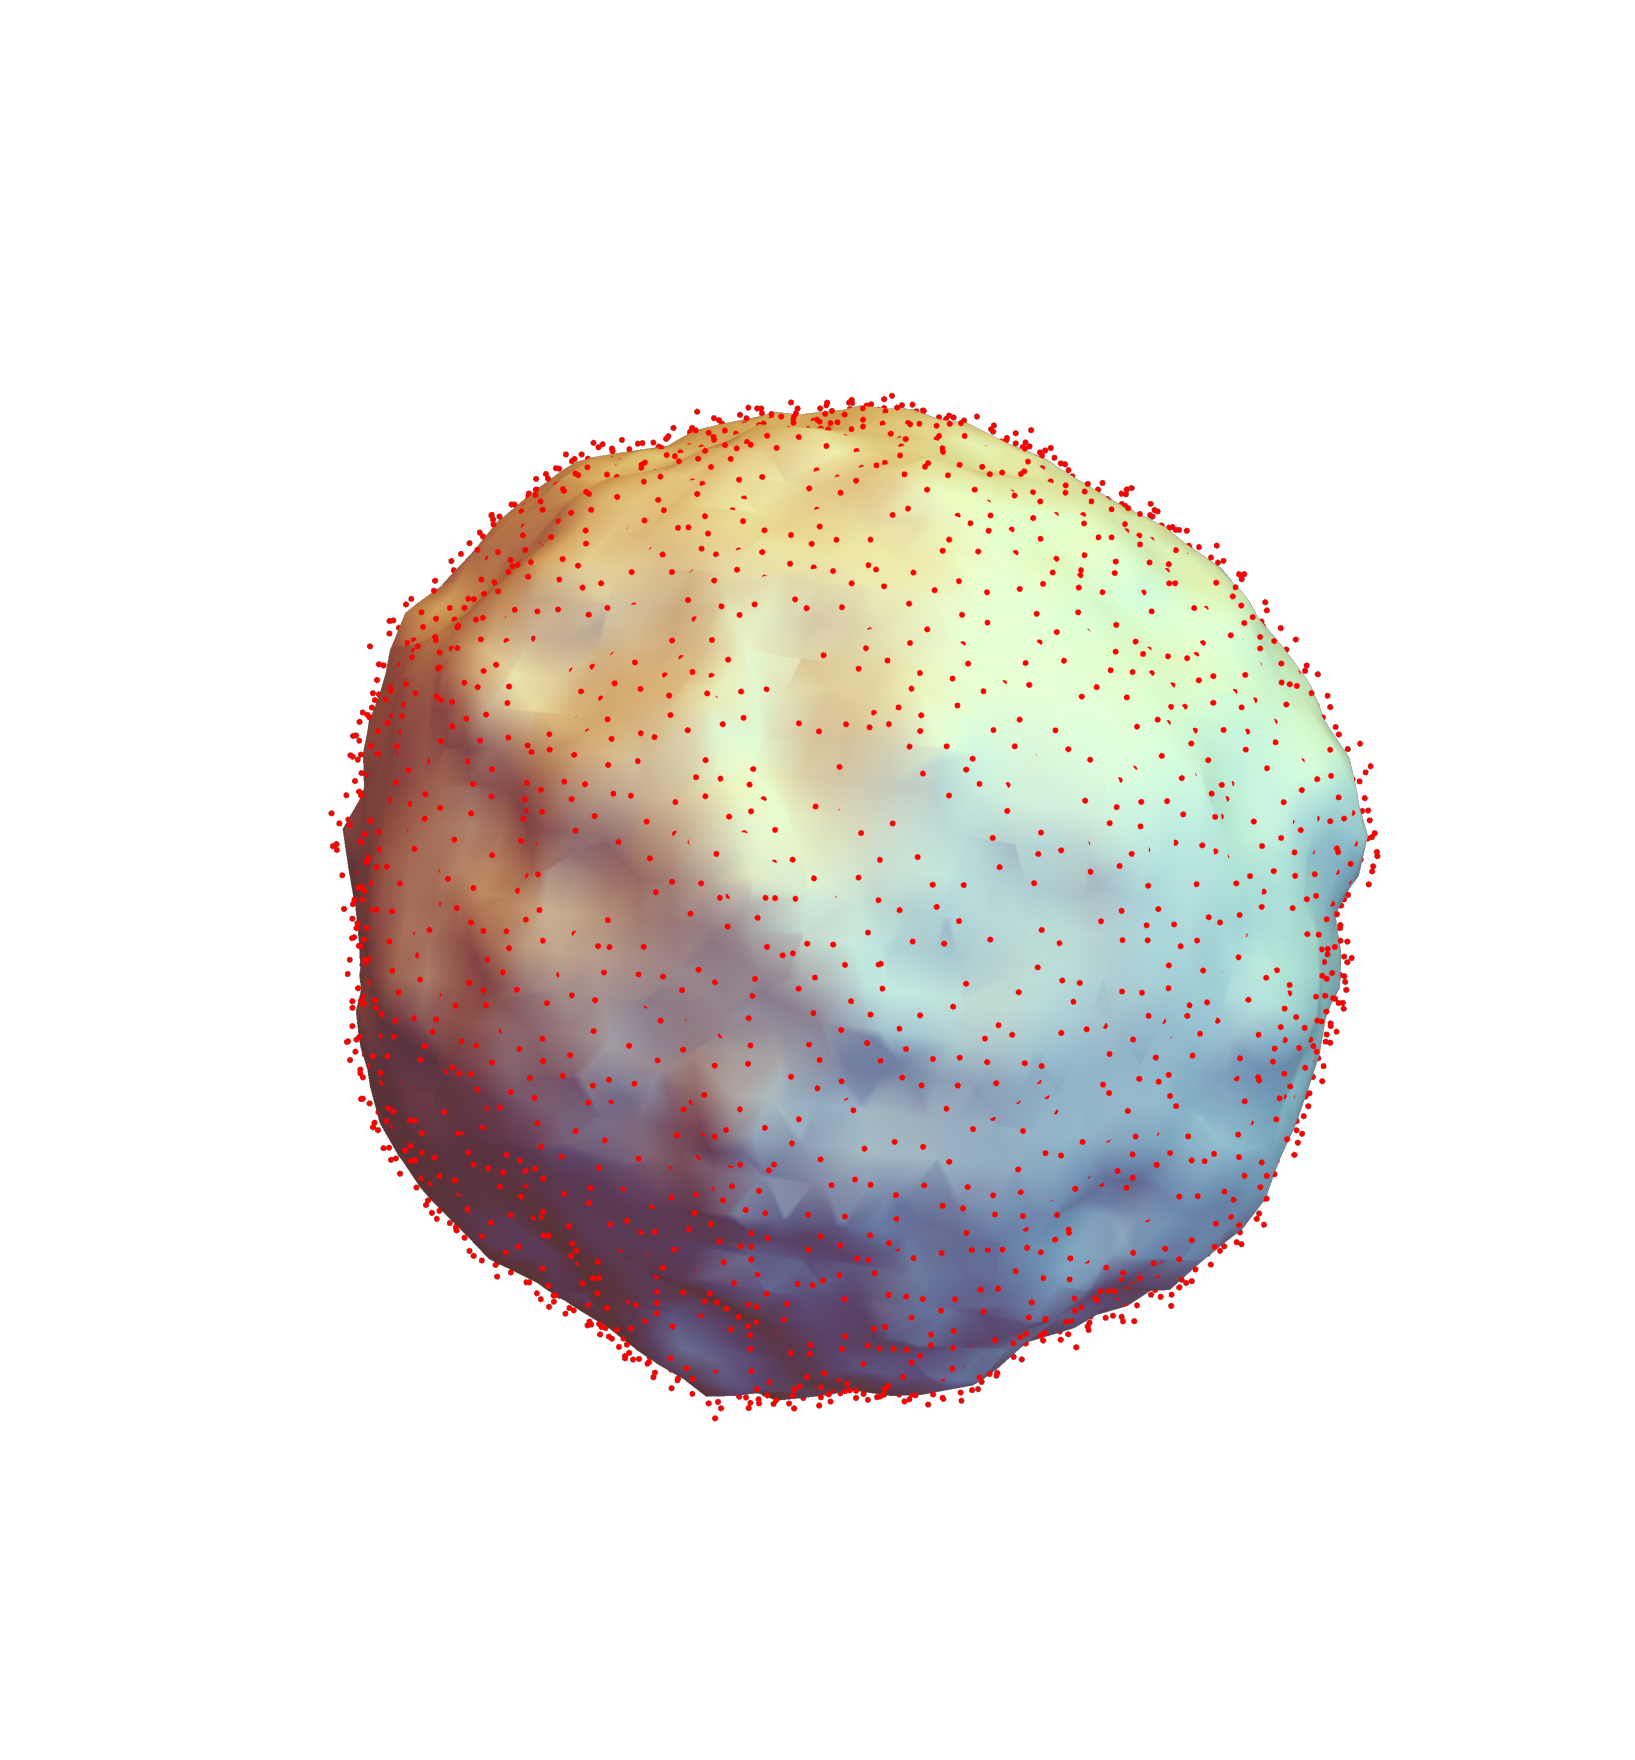
\includegraphics[width=1\linewidth,angle=0]{Fig10.pdf}
\caption{ The shape of our 3D membrane model at equilibrium. The red dots represent the particles in our 3D membrane model. The particles are triangulated and interact according to the Hamiltonian $H=\sum_{\rm faces}\left[ (k_A(A-A_0)^2 +\sum_{i=1}^3 k_\theta (\theta_i-\pi/3)^2 + \sum^\prime k_\phi (\phi-\pi)^2)\right]$, where $\sum_{\rm faces}$ is a sum over the triangulated faces, $A$ is the area of a triangulated face, $\theta_i$ are the angles inside a triangulated face,  $\sum^\prime$ denotes a sum over different adjacent phases and $\phi$ denotes the angle between two adjacent faces.}
\label{fig:3Dmembranesurface}
\end{figure*}
\begin{figure*}
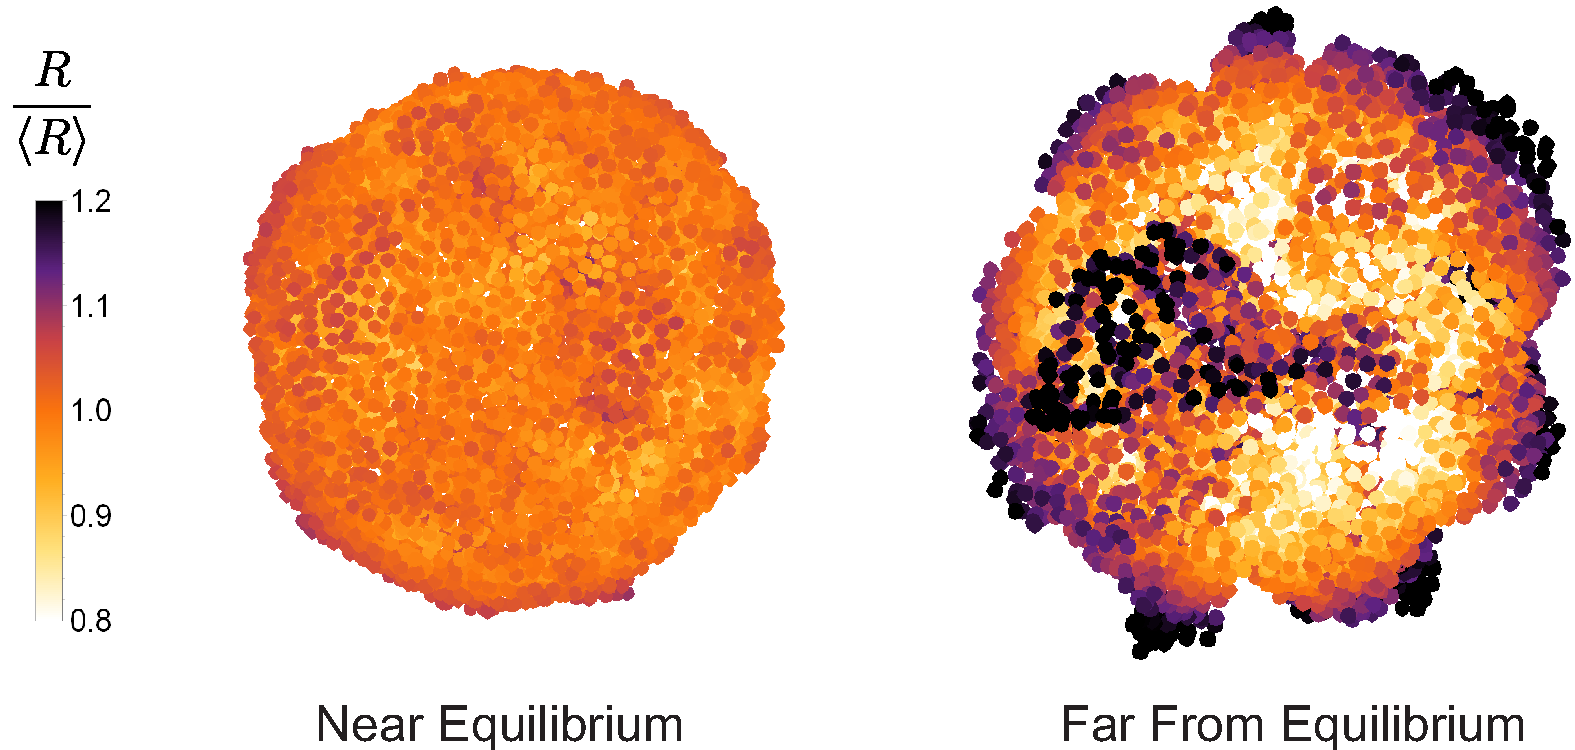
\includegraphics[width=1\linewidth,angle=0]{Fig11.pdf}
\caption{ A heat map detailing the deviations of particles from the averaged radius of the assembly. The heat map on the left is for the assembly near equilibrium. The heat map on the right is for the assembly far from equilibrium. The fluctuations in the heat map on the right are reminiscent of the buckling observed in the 2D model far from equilibrium}
\label{fig:relativeradius3D}
\end{figure*}
\begin{figure*}
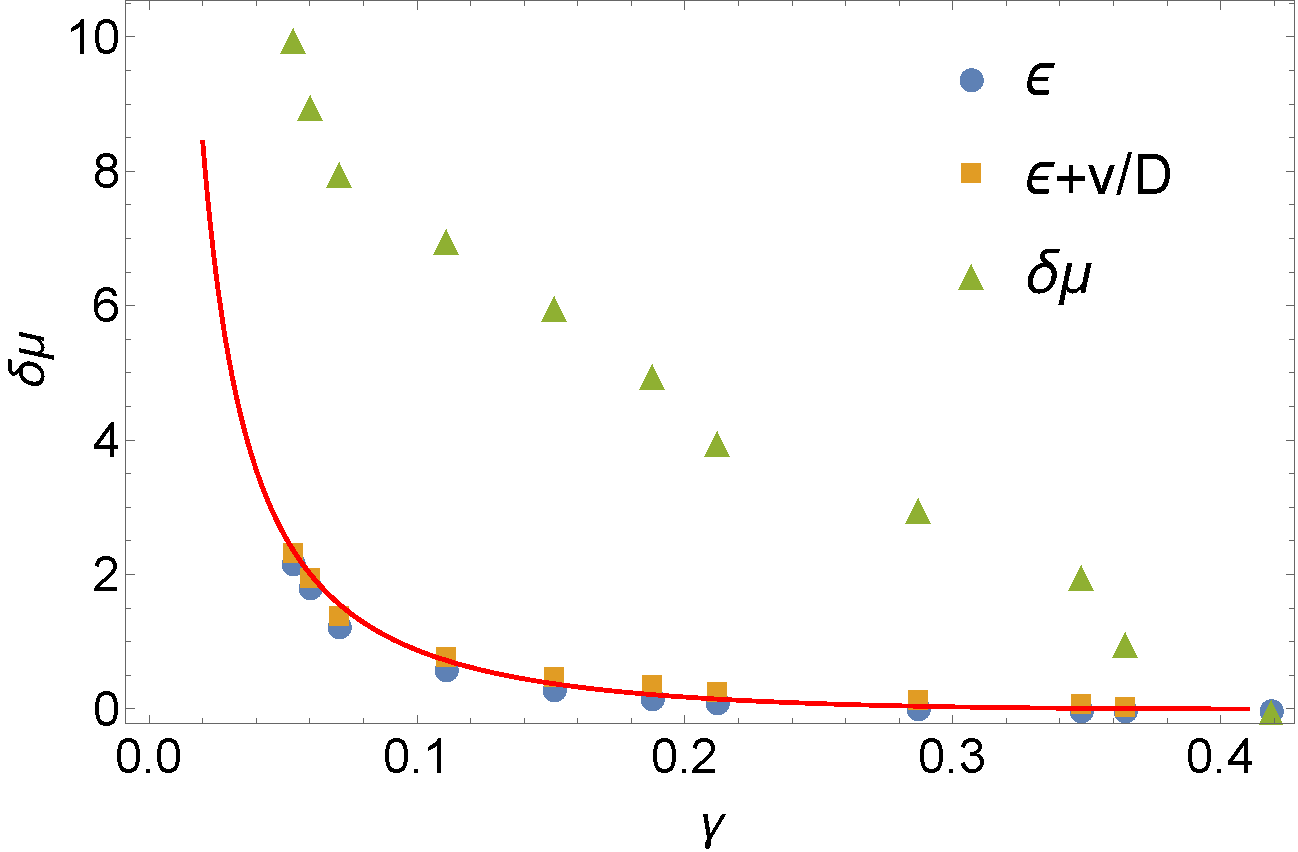
\includegraphics[width=1\linewidth,angle=0]{Fig12.pdf}
\caption{ This figure is similar to Fig. 6 in the main text but for 3D model. The reogranization cost $\epsilon_{\rm diss}$ is computed by decomposing the membrane fluctuations into spherical harmonic modes as explained in the text. We plan to further investigate these ideas in future work.}
\label{fig:boundsof3Dmembrane}
\end{figure*}
\bibliography{References02232018}
\end{document}